\documentclass[FM,BP]{tulthesis}

\usepackage[czech]{babel}
\usepackage[utf8]{inputenc}
\usepackage[a-1a]{pdfx}
\usepackage{hyperref}
\usepackage{amsmath}
\usepackage{amssymb}
\usepackage{nicefrac}
\usepackage{caption}
\usepackage{listings}

\usepackage[titles]{tocloft}
\usepackage[titletoc,title]{appendix}
\newcounter{Vzorce}
\addtocounter{Vzorce}{1}

\TULtitle{Řešení optimalizační úlohy LASSO pomocí proximálních algoritmů}{Solution to LASSO Using Proximal Algorithms}
\TULprogramme{B2646}{Informační technologie}{Information Technology}
\TULbranch{1802R007}{Informační technologie}{Information Technology}
\TULauthor{Václav Langr}
\TULsupervisor{doc. Ing. Zbyněk Koldovský, Ph.D.}

\begin{document}
\ThesisStart{male}{zadan}
\begin{acknowledgement}
Chtěl bych poděkovat vedoucímu této práce doc. Ing. Zbyňku Koldovskému, Ph.D. za velice přínosné konzultace, rady a trpělivost, bez kterých by tato práce nevznikla.
\end{acknowledgement}
\clearpage
\begin{abstractCZ}
Tato bakalářská práce je zaměřena na rekonstrukci řídkého vektoru z jeho komprimovaného pozorování. Pro rekonstrukci se využívá optimalizačního problému LASSO a jeho řešení pomocí proximálních algoritmů. Po vytvoření takového algoritmu, který je schopen původní signál rekonstruovat, se využívá metody Monte Carlo pro pozorování závislosti chyby řešení na parametru lambda. U takto získaného výpočtu je zjištěna kvadratická chyba řešení LASSO vzhledem k původnímu vektoru dat.


Vypracování bylo rozděleno do několika navazujících částí. Prvním a také nejdůležitějším krokem bylo nastudování vlastností proximálních algoritmů a výpočet proximálního operátora při různých vstupních funkcích. Po takto provedené rešerši proximálních algoritmů proběhla také rešerše vlastností optimalizační úlohy LASSO a jejích variant. V dalším kroku bylo možné přistoupit k implementaci algoritmu v programovacím jazyce a vývojovém prostředí MATLAB. Při postupné implementaci byl algoritmus upraven tak, aby vždy zkonvergoval ke správnému nebo alespoň co nejbližšímu přibližnému řešení optimalizačního problému. Z tohoto důvodu byl algoritmus rozšířen o podmínky optimality, jež ukončují výpočet při dosažení poměrně přesné aproximace. Dále byl algoritmus rozšířen o výpočet dynamické velikosti kroku, aby uživatel nemusel zadávat tento parametr, který velice ovlivňuje celkový chod algoritmu. S takto připraveným algoritmem mohla být použita metodika Monte Carlo k vytvoření numerické simulace, jež generuje nekomprimovaný řídký vektor dat, měřící matice s prvky, které mají Gaussovo rozložení a parametr lambda v zadaném rozsahu s logaritmickým rozdělením. Závěrečnou fází této práce bylo vytvoření metod vytvářející analytickou předpověď spolu s numerickou simulací pro rešeršní účely.


Zároveň tato práce navrhuje způsoby, jak může být pokračováno s nástroji, jež byly vytvořeny v průběhu jejího zpracování a získat tak přesnější výsledky.


\textbf{Klíčová slova:} MATLAB, proximální algoritmus, proximální operátor, LASSO, Monte Carlo
\end{abstractCZ}
\vspace{2cm}
\begin{abstractEN}
This bachelor thesis is focused on reconstruction of sparse vector from his compressed observation. For the reconstruction is used the LASSO problem and its solution using proximal algorithms. After creation of an algorithm that is able to restore the original signal is used Monte Carlo method for analyzing dependence of computation error on lambda parameter. Then is calculated the squared error for the found solution and the original data that is compared with the theoretical error.


Realization was divided into several parts. The very first and the most important step was studying the properties of proximal algorithms and evaluation of proximal operator for different functions. After the research on proximal algorithms there was also research on the properties of the LASSO and its variants. After that is was possible to implement algorithm using MATLAB language and development environment. The algorithm was modified during the implementation so it always converges into correct or at least approximate solution of LASSO. Due to this reason optimality conditions were added that terminates solving if the approximation is very accurate. Then was added a computation of dynamical step size that affects the whole algorithm so the user does not have to choose it. This prepared algorithm could be used for creation of Monte Carlo method that generates uncompressed sparse vector of data, random measurement matrix with Gaussian distribution and a lambda parameter within an interval with logarithmic distribution. The last step was to study Monte Carlo simulation and create methods for research purposes that would compute analytic prediction and numerical simulation.


The result of this thesis can be used for another usage. One of the possible usage is for example creation of a new data format. The compressed data would be saved in this format and only if the measurement matrix is not the same for all compressions it would be also saved. On the client side the original uncompressed signal would be recovered.


\textbf{Keywords:} MATLAB, Proximal Algorithm, Proximal Operator, LASSO, Monte Carlo
\end{abstractEN}
\clearpage
\tableofcontents

\listoffigures

\newcommand{\listequationsname}{Seznam vzorců}
\newlistof{myequations}{equ}{\listequationsname}
\newcommand{\myequations}[1]{%
	\addcontentsline{equ}{myequations}{\protect\numberline{}#1}\par}
\setlength{\cftmyequationsnumwidth}{0.0em}
\listofmyequations

\pagebreak

\renewcommand{\baselinestretch}{1.50}
\setlength\parindent{1.2cm}
\selectfont

\chapter{Úvod}
\label{ch:uvod}
 V dnešním světě, kdy získáváme stále více důležitých a velkých dat je stále větší nutností nějakým způsobem získaná data komprimovat. Z uvedeného důvodu se tato práce zabývá komprimovaným vzorkováním dat a následnou rekonstrukcí u koncového uživatele. Bude pro to použito nového přístupu rekonstrukce původních dat a to pomocí proximálních algoritmů, které jsou rychlé a jednoduché na implementaci.

Základní měření odpovídá funkci, viz \ref{eq:Zakladni mereni}, kde jsou původní data $x_0 \in \mathbb{C}^n$ transformována měřící maticí $A \in \mathbb{C} ^{m \cdot n}$, kde $m$ je počet řádků a $n$ počet sloupců matice a v poslední řadě je nutné uvažovat i náhodná data $z \in \mathbb{C}^m$. V této práci $z$ reprezentuje náhodný šum, který je přítomen při každém měření. Takto jsou získaná nová data $y \in \mathbb{C}^m$. V obecných případech platí, že $m \geq n$, ale v nich nedochází k žádné komprimaci dat, případně by i vzrostla velikost dat. Následná rekonstrukce by se tak redukovala pouze na spočtení inverzní, v případě obdélníkové matice pseudoinverzní, matice $A^{-1}$ a spočtení původních dat $x_0$. Tato bakalářská práce se zabývá případy, kdy $m < n$ a nelze tedy použít pseudoinverzní matici, která existuje, ale nemá požadované vlastnosti a musí tedy být použit jiný přístup.

\begin{equation} \label{eq:Zakladni mereni} \tag{Vzorec \theVzorce}
y = A \cdot x_0 + z
\end{equation}
\myequations{\ref{eq:Zakladni mereni} - Základní měření}
\stepcounter{Vzorce}

Dle pravidel lineární algebry tak existuje nekonečně mnoho řešení a je tudíž nemožné v tomto případě zrekonstruovat původní data. Nicméně ve skutečnosti lze data zrekonstruovat a to za podmínky, že původní vektor dat $x_0$ je řídký, tedy většina prvků z $x_0$ je rovna $0$. Právě z popsaného důvodu jsou kompresní algoritmy, například pro kompresi formátu JPEG, kdy se ukládají pouze největší koeficienty diskrétní kosinové transformace, tak efektivní. Popsaná podmínka není jedinou nutnou k úspěšné rekonstrukci. Další podmínkou je správně zvolená měřící matice $A$. Například, při volbě diagonální jednotkové matice, by komprimovaná data $y$ byla z velké části nulová. Z předestřeného důvodu by pak nebylo možné rekonstruovat původní data. Jelikož je toto téma velice zkoumané v celosvětovém měřítku, vzniklo mnoho výzkumů, které se touto problematikou zabývají velice podrobně. Právě výzkumy ve světě ukazují, že má-li dojít k jisté rekonstrukci, je možné využít měřící matice o náhodných prvcích z normovaného normálního rozdělení, tj. normální rozdělení s nulovou střední hodnotou a jednotkovým rozptylem. V následujících kapitolách budou probrány jednotlivé kroky, které vedou k úspěšné rekonstrukci dat.

\chapter{Optimalizační problémy}
\label{ch:optproblem}
Problém rekonstrukce původních dat z komprimovaného vzorkování se vyskytuje v nejrůznějších oborech.  Mezi tyto obory patří strojové učení, zpracování signálů a další. Jeden z možných přístupů je definovat tzv. optimalizační problém. Optimalizační problém je takový, kdy hledáme nejlepší možné řešení $x$ ze všech možných a to tak, aby $f(x)$ bylo maximální nebo minimální, podle zadané úlohy. Hledáme tedy globální maximum, respektive minimum, na průběhu křivky. 


Veškeré další řešení je založeno na tom, že lze optimalizační problémy zapsat v \textit{neomezeném} tvaru. V tomto tvaru se minimalizuje obecný vstup $x$ přes součet $m$ konvexních funkcích $f_0 \ldots f_m$, které náleží množině $\mathbb{R}^m$. Takto zapsaný problém by byl definován jako:

\begin{equation} \label{eq:Obecny problem} \tag{Vzorec \theVzorce}
\underset{x \in \mathbb{R}^n} {\mathrm{min}} f_{0}(x)+\ldots+f_{m}(x)
\end{equation}
\myequations{\ref{eq:Obecny problem} - Obecný optimalizační problém}
\stepcounter{Vzorce}

Nicméně, jelikož lze uvažovat jakoukoliv výše zmíněnou funkci, může se vyskytnout typický problém. Některé funkce nejsou diferencovatelné. Z tohoto důvodu se nadále bude na funkce a jejich řešení nahlížet jako na samostatný problém.

\section{Optimalizační problém LASSO}
\label{subch:optLASSO}
Jednou z variant jak řešit zadání této bakalářské práce je použití minimalizace a to tak, že se využije neomezeného tvaru optimalizačního problému pouze s funkcemi $f_0$ a $f_1$. Jedna z těchto funkcí se nahradí konkrétním předpisem pro rekonstrukci dat. Vznikne tak \ref{eq:Obecne LASSO}. Funkce $f_1(x)$ ve vzorci je libovolná a volí se podle toho, jaké vlastnosti mají vstupní data. 

\begin{equation} \label{eq:Obecne LASSO} \tag{Vzorec \theVzorce}
\underset{x} {\mathrm{argmin}} ~\left\{\left\|y-A \cdot x\right\| ^2 _2+ \lambda \cdot f_1(x)\right\}
\end{equation}
\myequations{\ref{eq:Obecne LASSO} - Obecná úloha LASSO}
\stepcounter{Vzorce}

V případě řídkého vektoru se volí taková funkce, která zajišťuje řídkost řešení. Jednou z možných funkcí, jež má tyto vlastnosti, je $\left\|x\right\|_1$ a vzniká tak vztah popsaný níže. Tento nový vztah zároveň řeší dva problémy a to rekonstrukci původních dat $x_0$ a jejich odšumnění.

\begin{equation} \label{eq:Konkretni LASSO} \tag{Vzorec \theVzorce}
\underset{x} {\mathrm{argmin}} ~\left\{\left\|y-A \cdot x\right\| ^2 _2+ \lambda \cdot \left\|x\right\|_1\right\}
\end{equation}
\myequations{\ref{eq:Konkretni LASSO} - Konkrétní úloha LASSO}
\stepcounter{Vzorce}

Jelikož obě funkce optimalizačního problému LASSO obsahují funkci normy, musí být zmíněna i její definice, která je popsána $\left\|x\right\|_p = \left(\sum_{i=1}^{n} \left|x_i\right|^p\right)^{1/p}$. V případě $\left\| \cdot \right\|_{1} $ tak získáme pouze sumu absolutních hodnot a vzniká současně problém, jak bylo naznačeno v kapitole \ref{ch:optproblem}, tedy nediferenciovatelná funkce. Jak je logické z definice absolutní hodnoty a derivace, lze sestrojit nekonečně mnoho tečen v bodě se souřadnicemi $[0, 0]$, v případě dvourozměrného prostoru, a nelze tak spočítat její derivaci v tomto bodě. Pro další zpracování je důležité uvědomění si, že funkce nemá derivaci a proto s ní musí být pracováno odlišným způsobem.

\chapter{Proximální algoritmy}
\label{ch:proxalg}
Jednou z možností, jak vyřešit optimalizační problém zmíněný v předchozí kapitole, je využít proximální algoritmy a proximální operátory příslušející konkrétním funkcím optimalizačního problému. Proximální algoritmus můžeme vhodně zapsat vztahem:

\begin{equation} \label{eq:proxAlg} \tag{Vzorec \theVzorce}
x_{n+1} = prox_{\lambda \cdot f}(x_{n})
\end{equation}
\myequations{\ref{eq:proxAlg} - Zápis proximálního algoritmu}
\stepcounter{Vzorce}

V tomto vzorci je $f$ uzavřená konvexní funkce, která splňuje $f : \mathbb{R}^{m} \rightarrow \mathbb{R} \cup \left\{+\infty\right\}$. Jelikož je proximální algoritmus založen na iteračním postupu, je to také zohledněno ve vzorci a to použitím indexu $n$. Pro $n+1$ iteraci platí, že se spočítá proximální operátor z $n$ kroku. Jak je vidno, proximální algoritmy jsou velice výhodné, pouze pokud je výpočet proximálního operátoru efektivní a velice rychlý na výpočet. Pokud by nebylo splněno toto kritérium, pak by se mnoho času strávilo výpočtem proximálního operátoru, který se musí provádět v každé iteraci algoritmu. Další výhodou těchto algoritmů je také to, že byly navrženy pro takové funkce, které musí být spojité, ale nemusí být diferencovatelné. Lze je tak využít pro velké množství obecných problémů.

\section{Proximální operátor}
\label{subch:proxOpt}
Jak již bylo naznačeno v úvodu této kapitoly, bude využito proximálního operátoru pro výpočet nového kroku proximálního algoritmu. Proximální operátory jsou velice důležitou součástí a to proto, že nahrazují funkce, které jsou obtížně řešitelné nebo by jejich výpočet byl velice zdlouhavý. V případě hladké funkce tedy dochází k postupnému nalezení globálního minima. 

Jelikož se v konkrétním předpisu úlohy LASSO, viz \ref{eq:Konkretni LASSO}, objevuje funkce $\left\| x\right\| _1$, musí být použit proximální operátor nazývaný \uv{měkké prahování}, dle \cite{proxAlg1} a \cite{proxAlg2}. Jedná se o velice jednoduchou funkci, kdy se vstupní data porovnávají s parametrem a to dle vztahu \ref{eq:soft}. 

\begin{equation} \label{eq:soft} \tag{Vzorec \theVzorce}
soft(x, \lambda) = \begin{cases}
0  & x \leq \lambda\\
x - \lambda & x > 0\\
x + \lambda & x < 0
\end{cases}
\end{equation}
\myequations{\ref{eq:soft} - Měkké prahování}
\stepcounter{Vzorce}
 
 Celkovou rychlost operátoru tedy určuje zejména parametr $\lambda$, o který se vstupní data mění v každém kroku. Parametry $\lambda$ nám tedy udává velikost změny od vstupních dat $x$. Pro lepší pochopení této funkce je zařazen graf \ref{fig:threshhold}, ve kterém se vstupní data z intervalu $\left\langle -5, 5\right\rangle $ změní maximálně o parametr $\lambda$, jenž byl zvolen $\lambda = 0,5$.
 
\begin{figure}[!ht]
\begin{center}
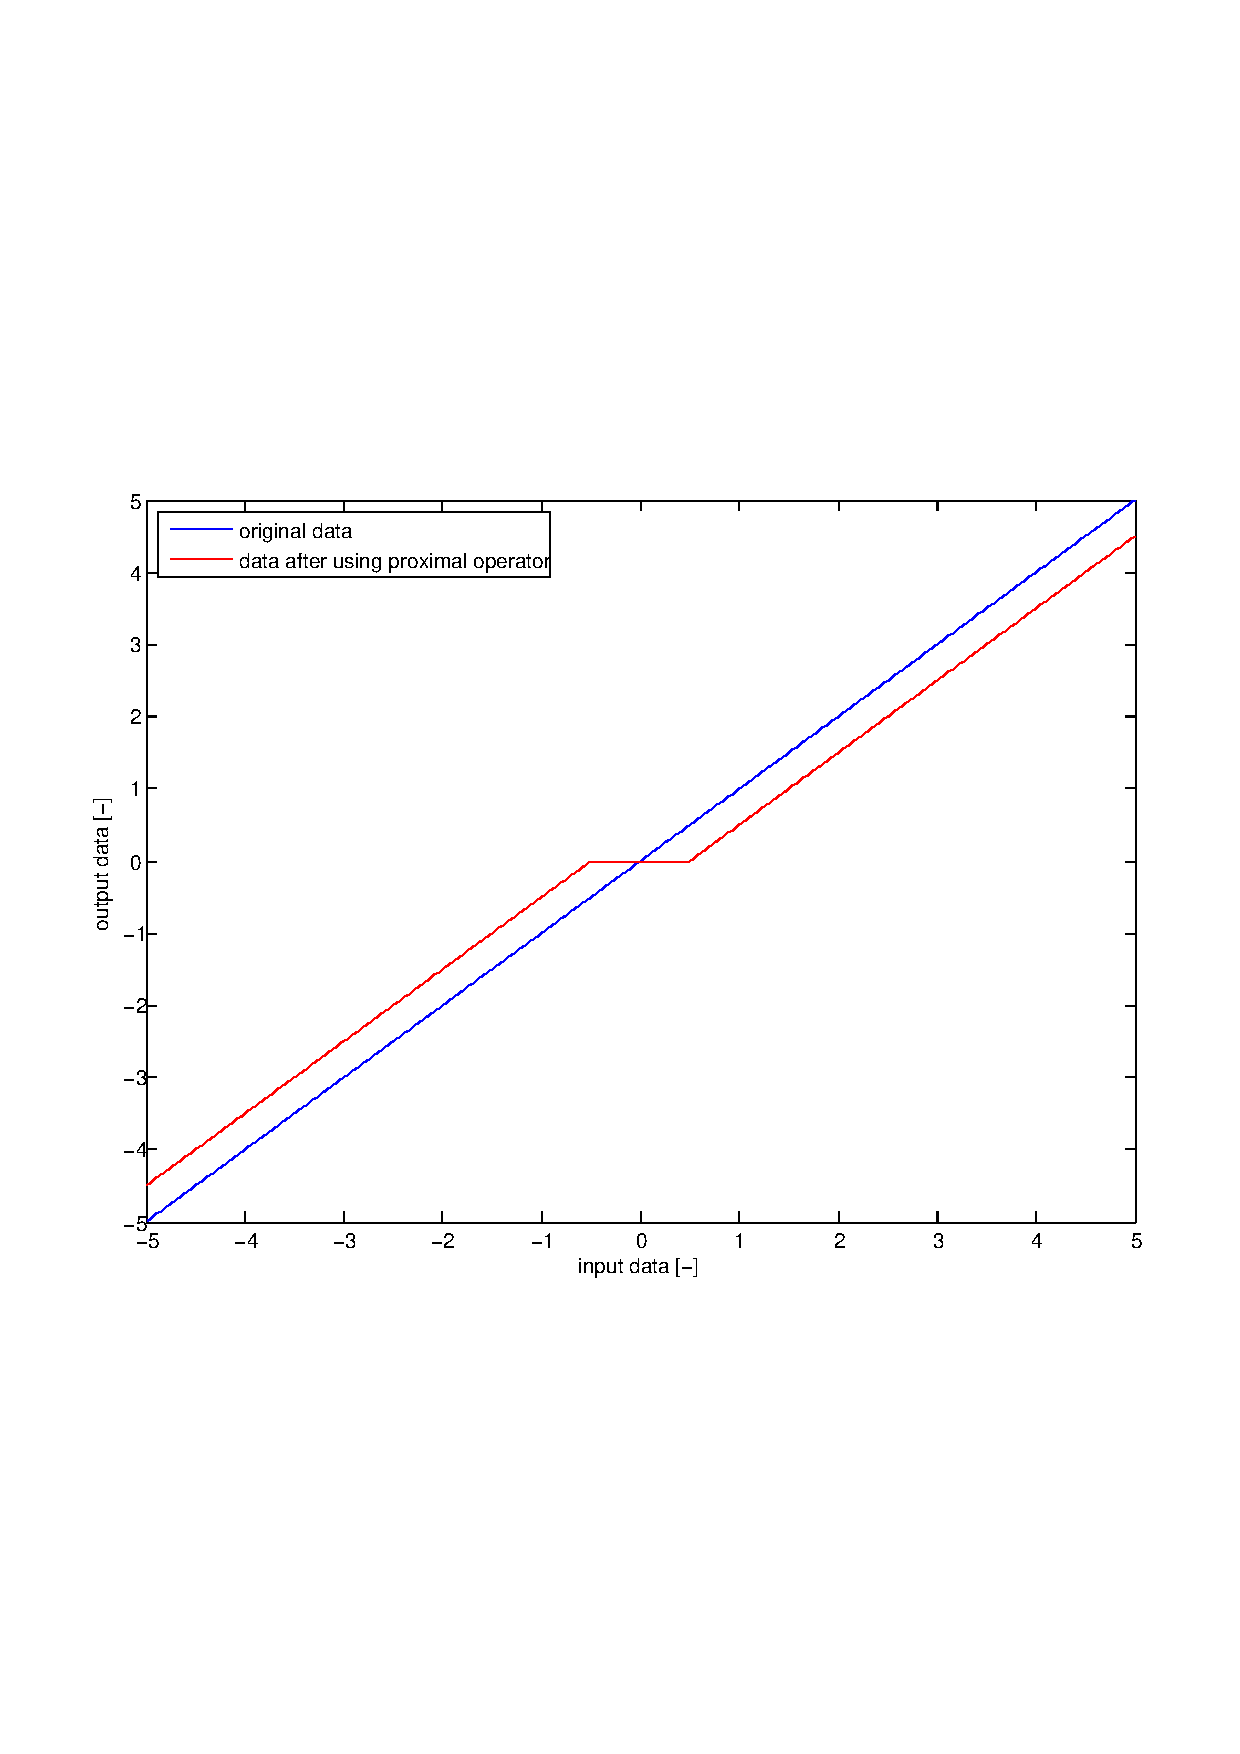
\includegraphics[scale=0.7]{obr/threshhold.pdf}
\end{center}
\caption{Průběh zvoleného proximálního operátoru pro $\lambda$ = 0,5}
\label{fig:threshhold}
\end{figure}

\chapter{Dopředno-zpětný algoritmus}
\label{ch:fwbw}
Jako hlavní algoritmus, na který se tato práce zaměřuje, je dopředno-zpětný algoritmus. Jeho základní varianta, popsaná obrázkem \ref{fig:fw-bw alg}, používá pevnou délku kroku. Je to iterační algoritmus, jež získá na vstupu komprimovaná data $y$, měřící matici $A$, velikost kroku $\alpha$ a kompenzační parametr $\lambda$, pro nějž chce uživatel získat konkrétní výsledek.
\begin{figure}[!ht]
\begin{center}
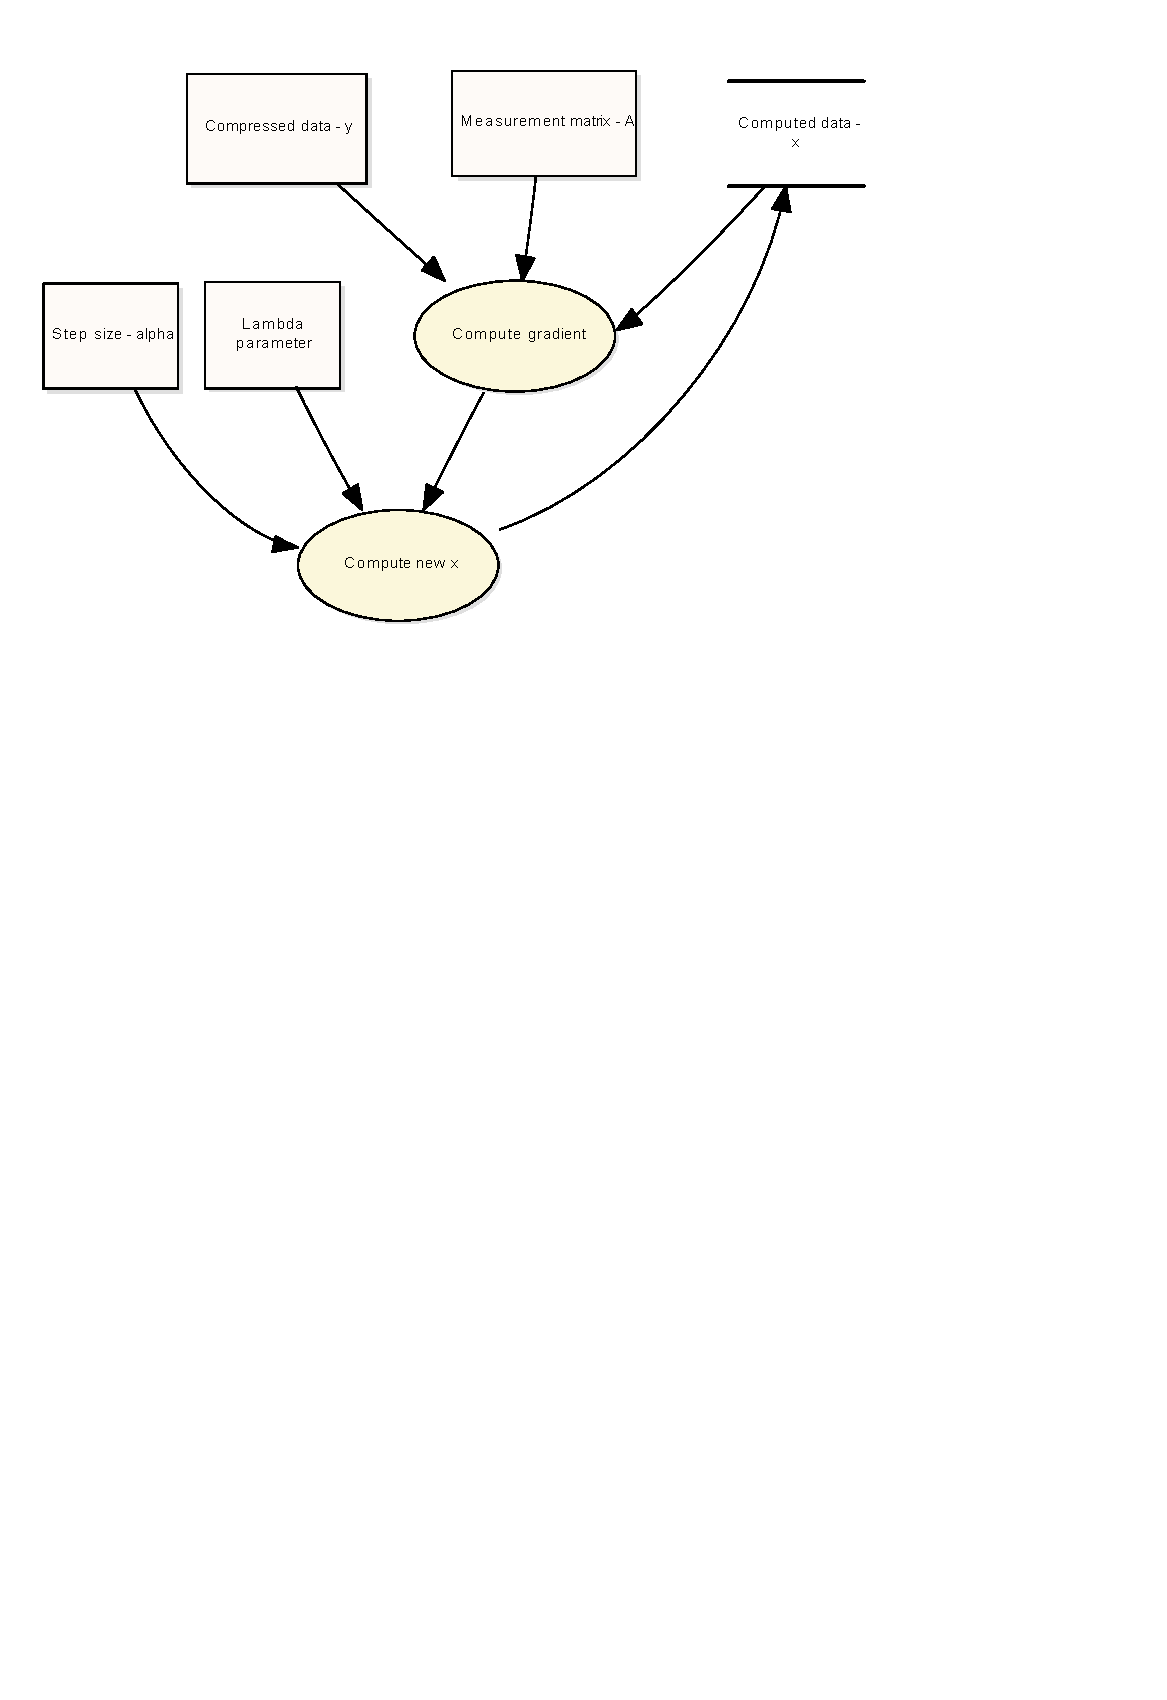
\includegraphics[scale=0.85]{obr/forwardbackward.pdf}
\end{center}
\caption{Schéma dopředno-zpětného algoritmu}
\label{fig:fw-bw alg}
\end{figure}

Za pomoci těchto údajů se v každém kroku počítá gradient diferencovatelné části optimalizační úlohy LASSO, v našem případě je to $\left|\right|y-A \cdot x\left|\right|_{2}^{2}$. Předpis zmiňovaného gradientu je funkce dle \ref{eq:GradientLASSO}.

\begin{equation} \label{eq:GradientLASSO}  \tag{Vzorec \theVzorce}
\partial f(x) = -2 \cdot A^T \cdot (y-A \cdot x)
\end{equation}
\myequations{\ref{eq:GradientLASSO} - Derivace funkce $\left\| y - A \times x\right\|_{2}^{2}$ }
\stepcounter{Vzorce}

Poté se již spočítá nový vektor dat $x$ za pomoci proximálního operátoru, jehož průběh byl znázorněn v předchozí kapitole, dle vzorce viz \ref{eq:ComputeX}. 

\begin{equation} \label{eq:ComputeX}  \tag{Vzorec \theVzorce}
x_{n+1} = prox_{\lambda \cdot \alpha}(x_{n}- \alpha \cdot \partial f(x_{n}))
\end{equation}
\myequations{\ref{eq:ComputeX} - Výpočet nových dat $x$}
\stepcounter{Vzorce}

Výpočet provedený dle předchozího kroku dává řešení postupně konvergující k optimálnímu bodu a to za předpokladu, že byl vhodně zvolen kompenzační parametr $\lambda$. V případě neoptimálně zvoleného parametru $\lambda$ je algoritmus daleko rychlejší než v případě s optimálněji zvoleným parametrem, ale tolerance je příliš veliká, takže nedochází k úplné konvergenci. Vlivem špatné konvergence jsou získána nepřesná data.

Pro praktickou ukázku byly vytvořeny grafy v obrázku \ref{fig:basicLambda}. Pro tyto ukázky byly použity dva parametry $\lambda$, $100$ a $0,1$. Následně byly náhodně vygenerovány: vektor dat $x$, měřící matice $A$ a náhodný šum $z$. Uvedené proměnné byly shodné pro oba parametry $\lambda$. S takto zvoleným parametrem je průběh velice rychlý a v cca 100 iteracích je algoritmus ukončen. S druhou hodnotou parametru, $\lambda = 0,1$, není algoritmus tak rychlý, jako v předchozím případě, proběhne cca 1500 iterací algoritmu, ale jsou získána velice přesná data.

\begin{figure}[!ht]
	\begin{center}
		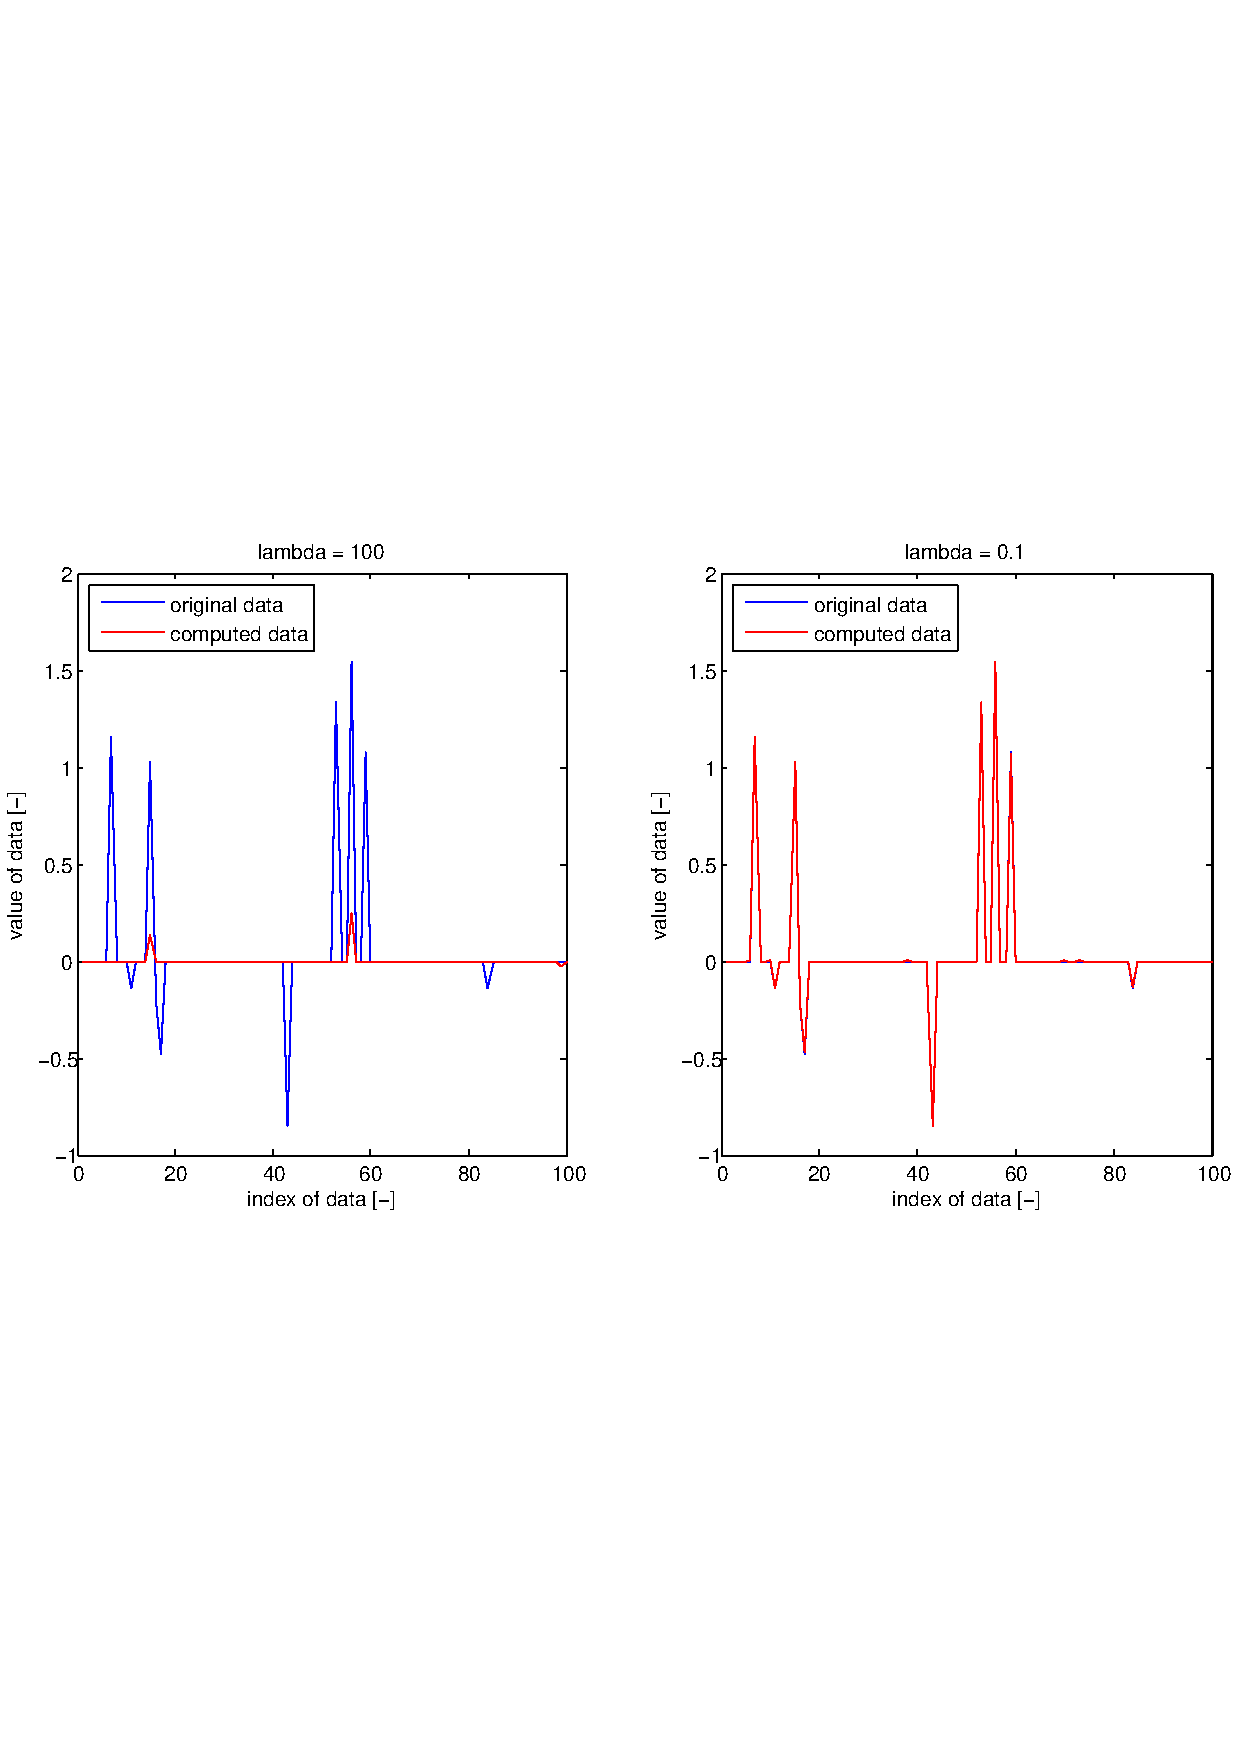
\includegraphics[scale=0.72]{obr/lambda.pdf}
	\end{center}
	\caption{Ukázka průběhu algoritmu při nevhodně zvoleném parametru $\lambda$}
	\label{fig:basicLambda}
\end{figure}

Jak je vidno z předložených grafů, je parametr $\lambda$ velice významný. V prvním případě, kdy byl parametr zvolen extrémně nevhodně, algoritmus nedokázal najít přesné řešení, jelikož tolerance algoritmu je příliš velká. Dokázal najít pouze část původních dat s redukovanou hodnotou a dokonce pro jeden prvek nezkovergoval vůbec k nule. Ve druhém případě již bylo nalezeno daleko přesnější řešení a nedošlo k chybnému nalezení prvku jako v předchozím případě.


\section{Délka kroku algoritmu}
\label{subch:dynamicStep}
Neméně významným parametrem, jako byl uvedený parametr $ \lambda $, je i délka kroku $ \alpha $. Pro pochopení fungování byl nejprve implementován algoritmus s pevnou délkou kroku. Ukázalo se, že toto není zcela optimální, jak bude naznačeno v následujících grafech.

\begin{figure}[!ht]
\begin{center}
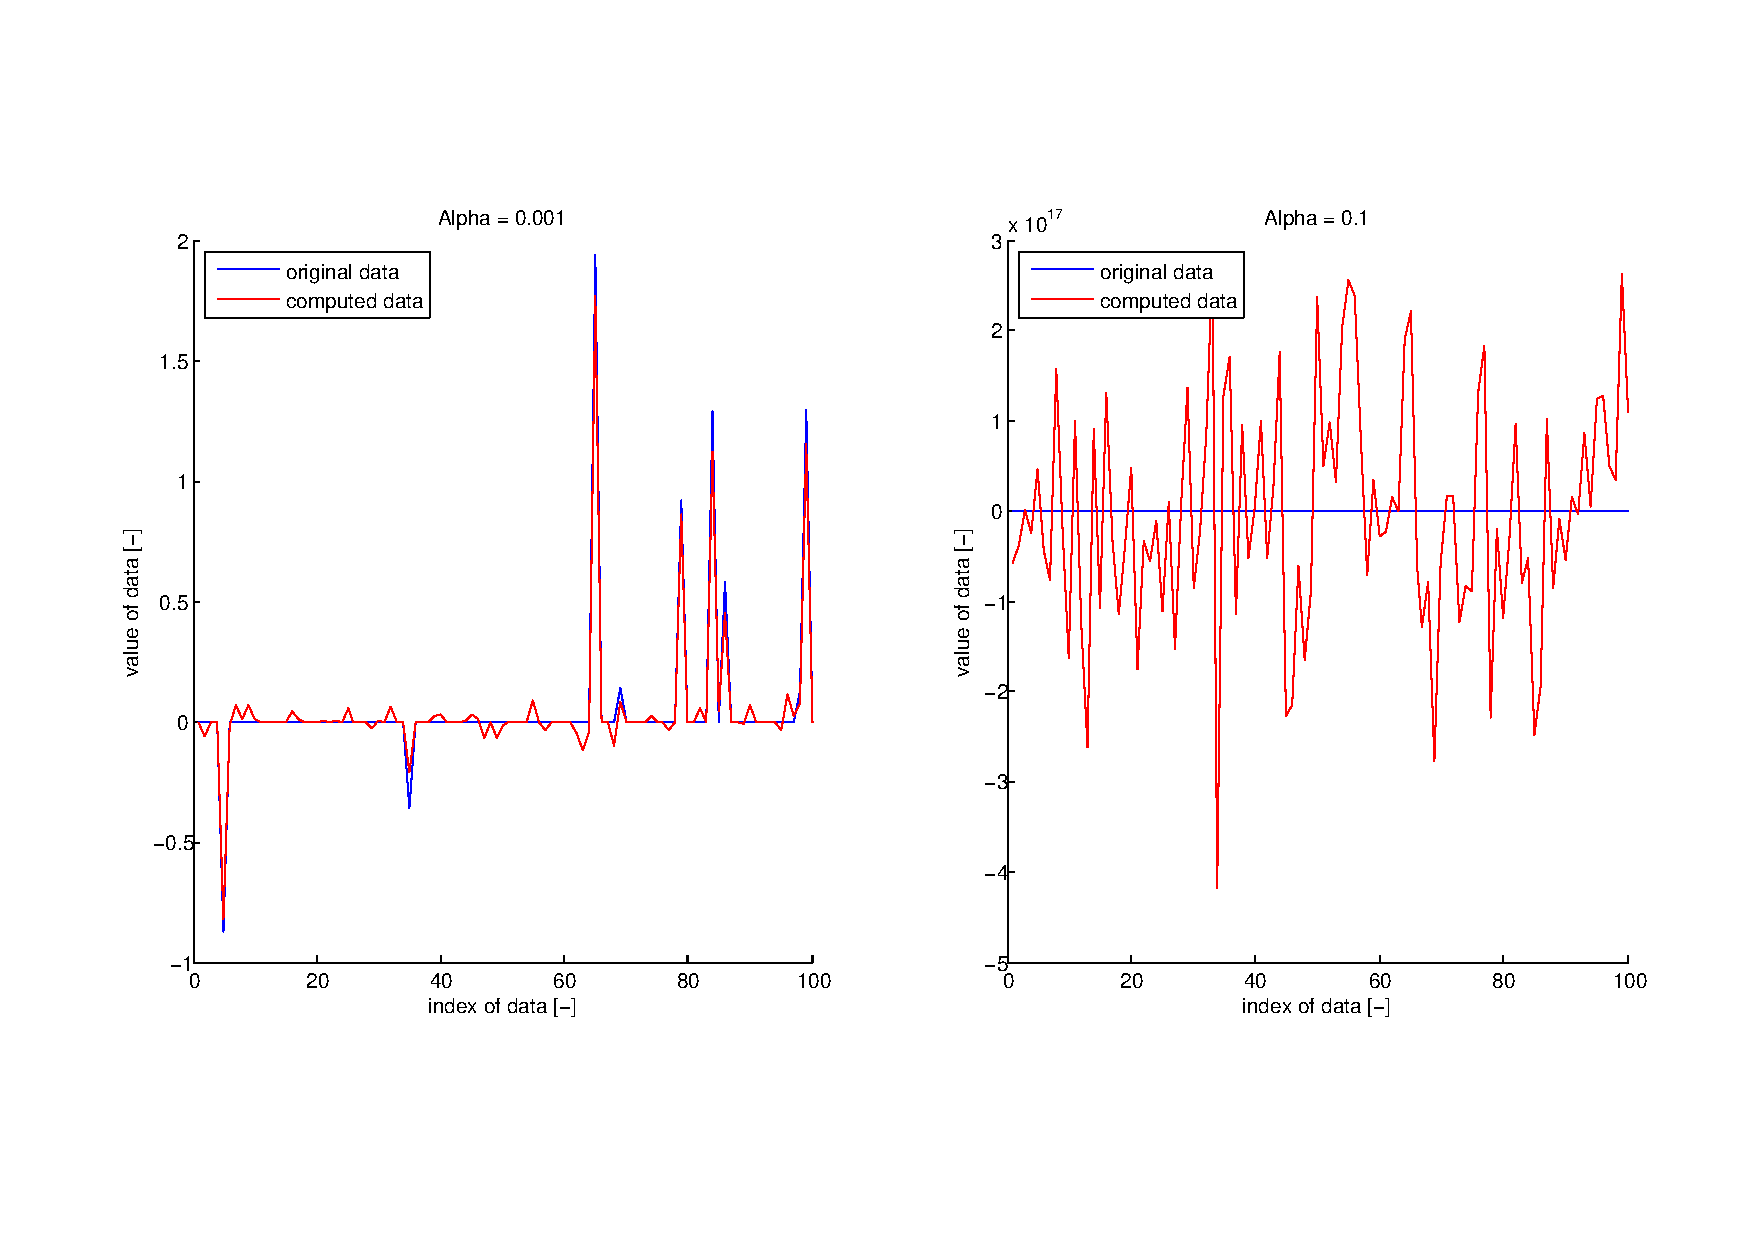
\includegraphics[scale=0.55]{obr/basic.pdf}
\end{center}
\caption{Ukázka průběhu algoritmu při různé volbě délky kroku}
\label{fig:basicAlpha}
\end{figure} 

Jak lze vidět grafech \ref{fig:basicAlpha} na následující stránce, tak délka kroku má obrovský dopad, dokonce větší než kompenzační parametr $\lambda$. Na levém grafu, pro jehož vytvoření byla použita přiměřená délka kroku algoritmu tj. $0,001$, je vidět, že algoritmus konverguje ke správnému řešení. Vzniká ale současně mnoho nepřesností, které se nepodařilo odstranit do konce průběhu algoritmu. V daném případě bylo nastaveno maximálně 5000 iterací. 

Pro názornost jsou uvedeny grafy, které představují v prvním případě změnu po jedné iteraci, jak je znázorněno v příloze C - obrázek \ref{fig:diff1}, konkrétně mezi 30 a 31 iterací. Druhá ukázka, viz příloha D - obrázek \ref{fig:diff300}, představuje změnu mezi 100 a 400 iterací. 

Ve druhém průběhu, kde byla použita stejná data jako v prvním grafu, lze vidět, že se algoritmus chová velmi citlivě. Proběhlo pouze deset iterací a řešení velice rychle diverguje. Z tohoto důvodu byl původní algoritmus rozšířen o dynamický výpočet velikosti kroku.

Dynamická volba kroku využívá přístupu z článku \cite{dynamickyKrok}, kdy se velikost kroku vypočte pomocí aktuálně nalezených $x_{n}$, předchozích dat $x_{n-1}$ a měřící matice $A$ dle vztahu \ref{eq:ComputeAlpha}.

\begin{equation} \label{eq:ComputeAlpha}  \tag{Vzorec \theVzorce}
\alpha = \frac{\left\| A \cdot (x_{n} - x_{n-1}) \right\|}{\left\| A^{T} \cdot A \cdot (x_{n} - x_{n-1}) \right\| }
\end{equation}
\myequations{\ref{eq:ComputeAlpha} - Výpočet délky kroku $\alpha$}
\stepcounter{Vzorce}

Nově upravený algoritmus již korektně rekonstruuje původní data, jak lze také vidět na grafu \ref{fig:dynamicAlpha} a je možné přistoupit k další části řešení této bakalářské práce.

\begin{figure}[!ht]
\begin{center}
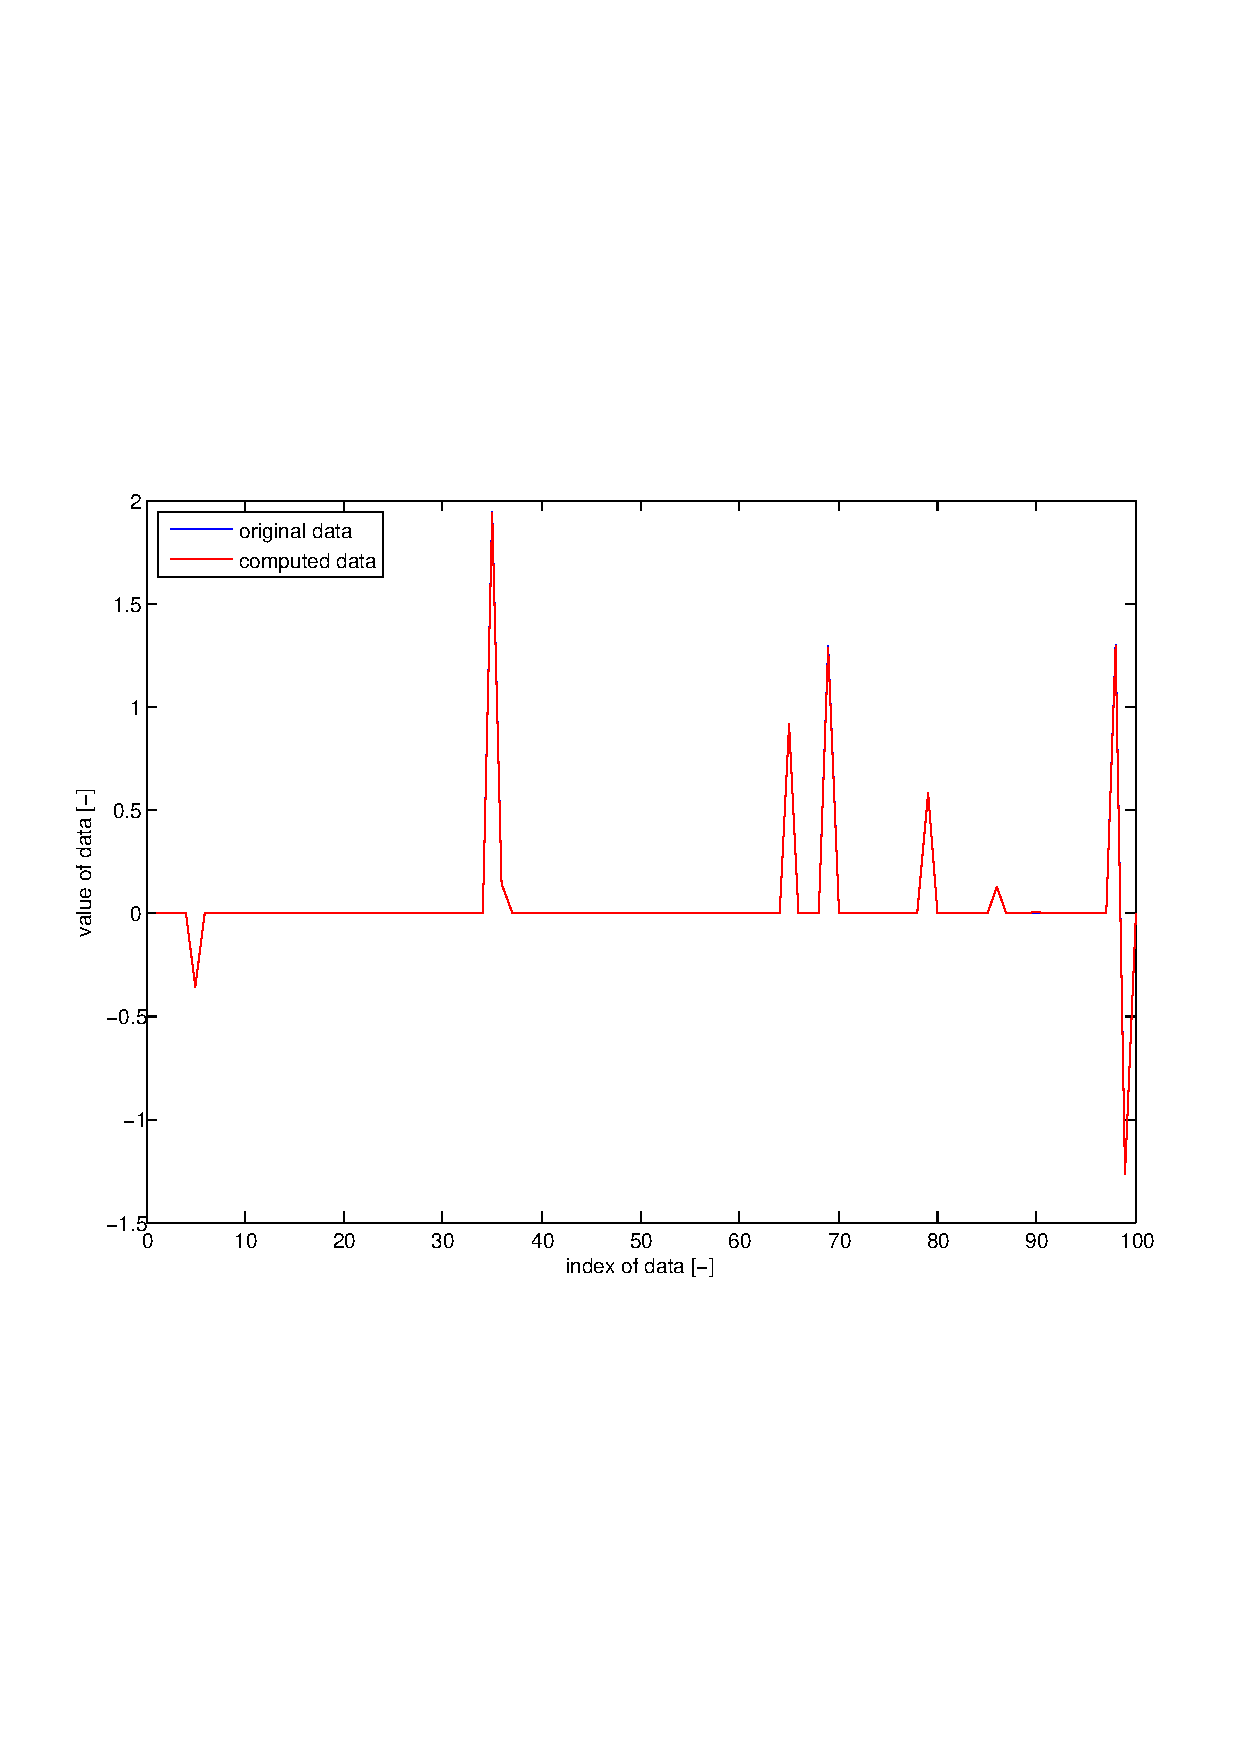
\includegraphics[scale=0.7]{obr/dynamic.pdf}
\end{center}
\caption{Ukázka průběhu algoritmu s dynamickou délkou kroku}
\label{fig:dynamicAlpha}
\end{figure}

\section{Podmínky optimality}
\label{subch:stopCrit}
Algoritmus připravený dle popisu v této kapitole byl dále rozšířen o podmínky optimality, které zaručují ukončení algoritmu, pakliže je změna rekonstruovaných dat dostatečně malá. Nadále uvažujeme podmínky pouze pro $\left\| \cdot \right\|_{2}^{2} $ LASSO, jelikož pro ostatní případy, které budou zmíněny v dalších kapitolách, tyto podmínky neplatí. V případě, že by algoritmus toto neobsahoval, došlo by v lepším případě pouze k nezastavení algoritmu a uživatel by pouze plýtval výpočetním časem. V horších případech by však mohlo dojít i k divergenci algoritmu z jakéhokoliv aktuálního bodu a to kvůli dynamické volbě kroku. 

Dynamická volba kroku je založena na výpočtu rozdílu aktuálního a předchozího kroku algoritmu. Pokud by tato změna byla dostatečně malá, vlivem nepřesnosti počítače by tak vznikla data obsahující pouze $0$ a právě z popsaného důvodu by se z původního výpočtu, viz \ref{eq:ComputeAlpha}, stalo $\nicefrac{0}{0}$, což je v oboru reálných čísel $\mathbb{R}$ nereálná možnost. Z předestřeného důvodu by došlo k chybě algoritmu a došlo by ke ztrátě aktuálního vypočteného signálu dat již při výpočtu bližšího bodu k optimálnímu. Právě kvůli těmto případům bylo využito článku \cite{homotopy}.

První z podmínek je $(a_{i}^{n})^{T} \cdot (A^{n} \cdot x^{n} - y^{n}) = - w_{i} \cdot z_{i}$. Ta se zabývá pouze nenulovými prvky z $n$ kroku proměnné $x^{n}$. V tomto případě se rozdíl aktuálního kroku komprimovaného vzorkování $A^{n} \cdot x^{n}$ a původního komprimovaného vzorkování $y^{n}$ vynásobený $a_{i}$, tedy $i$ sloupci matice $A^{n}$, porovnává s váhami $w_{i}$, které jsou navíc upraveny o znaménko $z_{i} = sign(x_{i}^{n})$.

Druhá z podmínek je velice podobná, ale zabývá se pouze nulovými prvky. Její definice je $\left|(a_{i}^{n})^{T} \cdot (A^{n} \cdot x^{n} - y^{n})\right| < w_{i}$. Porovnává se tedy, jestli je absolutní hodnota rozdílu aktuálně nalezeného komprimovaného vzorkování od původního komprimovaného vzorkování vynásobeného $i$ sloupci z matice $A$, kde $i$ značí indexy nulových prvků aktuálně nalezeného řešení $x^{n}$ menší než zadaná váha významnosti $w_{i}$.

V návaznosti na popsaný problém byly vytvořeny další dvě funkce pro uvedené podmínky. První z nich se zabývá pouze nenulovými prvky s indexy $i$ a má předpis:

\begin{equation} \label{eq:homotopy1}  \tag{Vzorec \theVzorce}
A_{i}^{T}\cdot(A \cdot x_{n} - y) + \lambda \cdot sign((x_{n})_{i}) < \epsilon
\end{equation}
\myequations{\ref{eq:homotopy1} - Podmínka optimality pro nenulové prvky}
\stepcounter{Vzorce}

Výsledek levé strany tohoto vzorce je porovnáván s uživatelem zadanou hodnotou $\epsilon$, což je velikost odchylky chyby, typicky je to velice malé číslo na hranici přesnosti datového typu. Tento vzorec byl následně upraven pro námi požadované konkrétní řešení, jelikož článek, ze kterého bylo čerpáno, uvažoval i různé parametry $\lambda$ pro každý prvek původních dat $x$. První z uvedených vzorců používal pouze nenulové hodnoty, muselo tedy být využito i druhé varianty vzorce pro nulové hodnoty a to ve tvaru:

\begin{equation} \label{eq:homotopy2}  \tag{Vzorec \theVzorce}
\left|A_{i}^{T} \cdot (A \cdot x_{n} - y)\right| < \lambda
\end{equation}
\myequations{\ref{eq:homotopy2} - Podmínka optimality pro nulové prvky}
\stepcounter{Vzorce}


\section{Konečná verze algoritmu}
\label{subch:finalAlg}
Po vypracování těchto kroků mohl být původní algoritmus, jehož diagram byl znázorněn v kapitole \ref{ch:fwbw}, upraven do konečné podoby. Po přidání funkčních bloků popsaných v předchozích podkapitolách, vypadá jeho diagram tak, jak je zobrazeno diagramem v příloze této práce. Konečná podoba je navržena tak, aby případná změna byla snadno proveditelná a bylo možné algoritmus dále rozšiřovat pro jiné účely případně i různé varianty optimalizační úlohy LASSO, např. využít různých kriteriálních podmínek. Zároveň se tímto rozšířením dosáhlo toho, že algoritmus vždy konverguje ke správné rekonstrukci a v případě divergence se okamžitě zastaví. 

Popsané řešení je jen dílčím výsledkem této práce, dosud nebylo uvažováno o závislosti kvadratické chyby rekonstrukce na zvoleném parametru $\lambda$. Proto bylo nutné zabývat se vytvořením metody, která bude schopná provést algoritmus na větším souboru dat, zároveň vypočte normovanou kvadratickou chybu a zajistí výpočet analytické předpovědi.

\chapter{Analýza chyby řešení}
\label{ch:simulace}
Aby bylo možné učinit obecně jakýkoliv závěr, v tomto případě pozorovat závislost parametru $\lambda$ a kvadratické chyby nalezeného řešení optimalizačního úlohy LASSO pomocí algoritmu navrženého v kapitole \ref{ch:fwbw}, je nutné vytvořit simulaci. Takovéto simulace vycházejí z metodiky, kdy se opakovaně provádí vybraný algoritmus na větším množství vygenerovaných dat, která jsou na sobě nezávislá a následný průměr kroků simulace poskytuje nástroj pro učinění závěru.

V tomto případě se simuluje získání dat $x$, která mohou pocházet z libovolného měření. Poté se opakovaně generuje náhodná měřící matice $A$ a následně se spočte komprimovaný vektor $y$, ke kterému je také přičten náhodný šum $z$. Tyto dvě proměnné jsou použity jako vstup pro zvolený algoritmus spolu s předem danými parametry $\lambda$ s logaritmickým rozložením v daném rozsahu, ve kterém je nutné sledovat závislost kvadratické chyby rekonstruovaných dat na uvedeném parametru $\lambda$.

\section{Realizace simulace}
\label{subch:sim}
Jednou z možných simulací je metoda Monte Carlo. Tato metoda je jednoduchá na realizaci, poskytuje velice přesné výsledky a zároveň splňuje veškeré nároky, které jsou požadovány od podobné simulace. Právě proto je vhodná pro prvotní testování daného algoritmu. 

Uvedená simulace je založena, jak již bylo zmíněno, na opakovaném generování náhodných dat, na kterých se provádí daný algoritmus a jsou takto získávány průběžné výsledky. Nicméně dílčí výsledky neříkají nic o celkové závislosti kvadratické chyby nalezeného řešení od původních dat na parametru $\lambda$ a proto jsou dílčí výsledky zprůměrovány. Následný průměr poté poskytuje empirické pozorování. Z tohoto pozorování již lze vyvodit optimální parametr $\lambda$. Ten představuje globální minimum průměru dané simulace. Uvedený parametr $\lambda$ je hledán pomocí simulace, protože neexistuje způsob, jak ho určit analyticky.

\begin{figure}[!ht]
	\begin{center}
		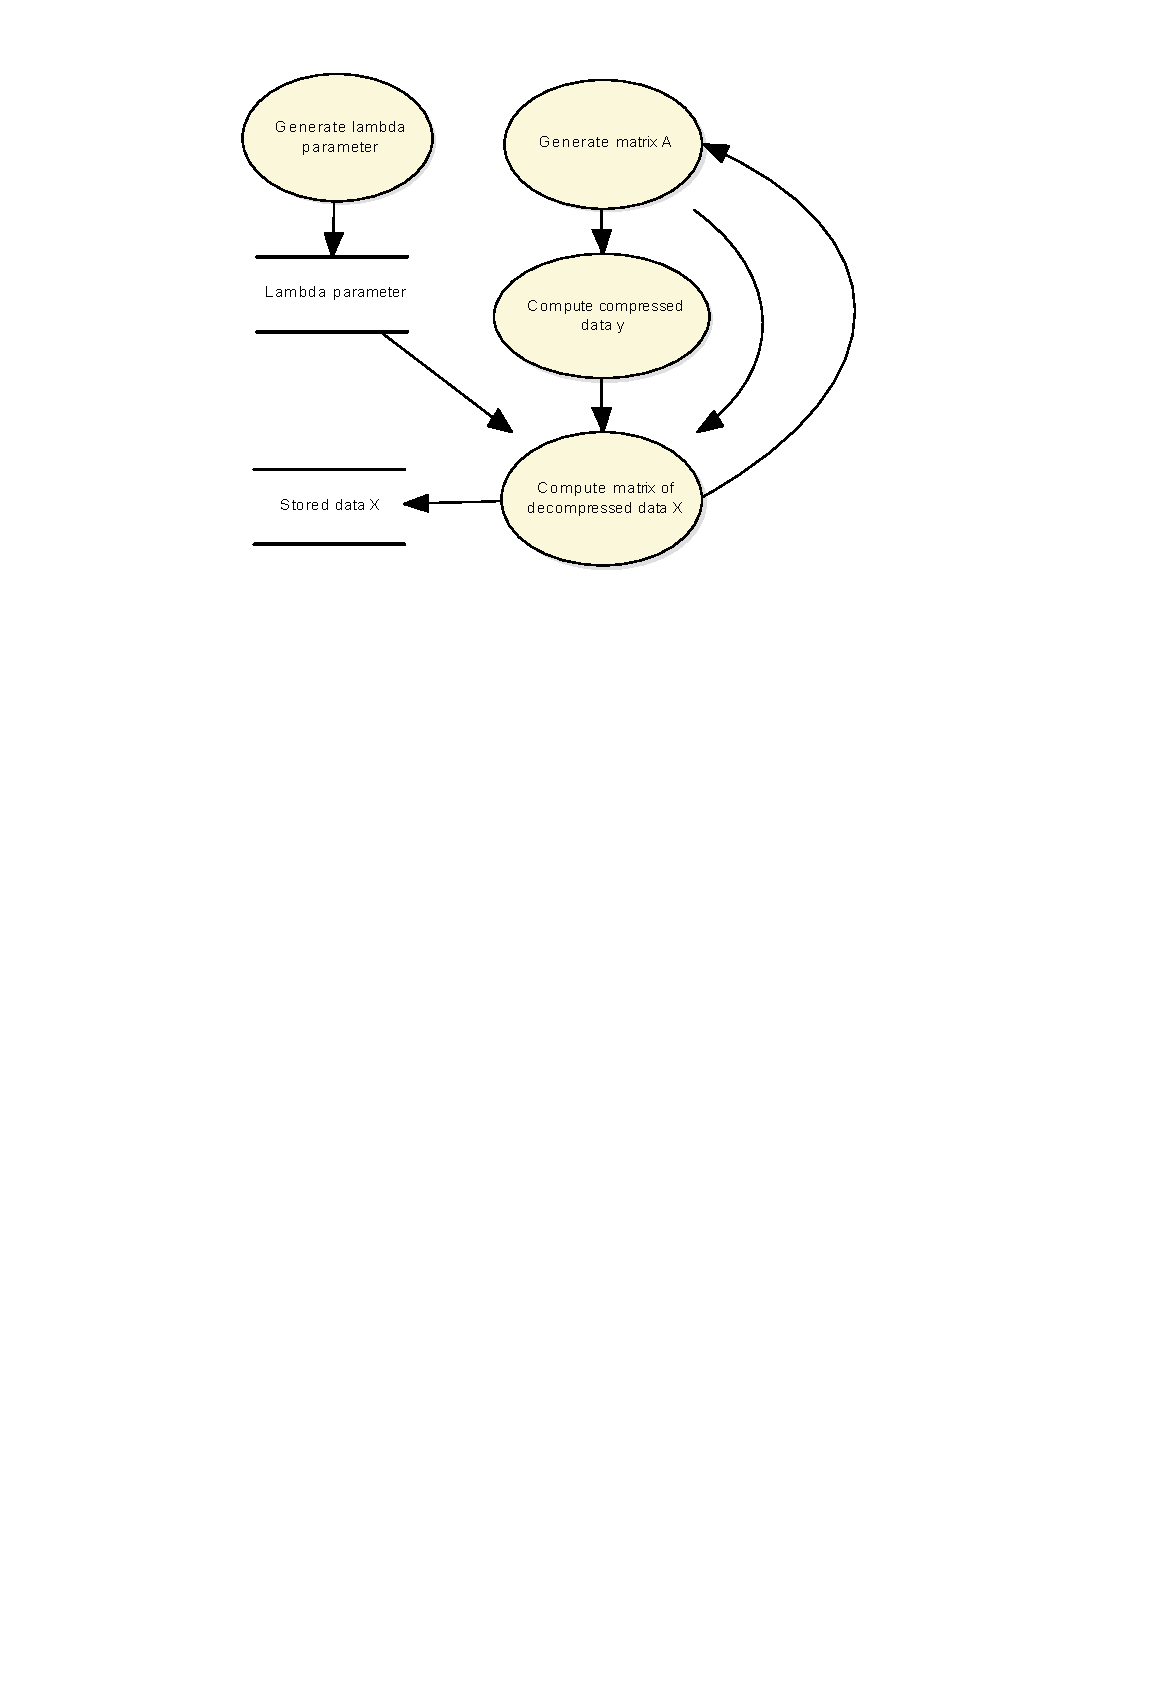
\includegraphics[scale=0.9]{obr/mcsim.pdf}
	\end{center}
	\caption{Simulace Monte Carlo}
	\label{fig:mcSim}
\end{figure}

Protože jde pouze o opakované provádění testovaného algoritmu, je tato simulace velice jednoduchá na realizaci. Základní algoritmus lze popsat diagramem \ref{fig:mcSim}. Nicméně jakákoliv takováto simulace má obrovskou nevýhodu a tou je celkový čas simulace. Při větších datech může výpočet trvat i několik dní na běžně dostupném výpočetním stroji. V případě uvedené konkrétní simulace se 100 prvky $\lambda$ a 1000 opakování trvá tato simulace pro $\left\| \cdot\right\|_{2}^{2} $ LASSO přes jedenáct hodin. Pro porovnání byl algoritmus upraven pro $\left\| \cdot \right\|_2 $ LASSO, které bude použito v dalších kapitolách této práce. Takováto simulace již trvá přes tři dny. Jelikož je vše realizováno pomocí vývojového prostředí a jazyku MATLAB, jednou z možností bylo vytvořit knihovní funkce v jazyku C nebo C++, aby se docílilo zrychlení algoritmu a využít této knihovny funkcí místo skriptů v MATLABu.  

Obdobou této možnosti bylo použití modifikované verze jazyka C++ s knihovnami pro programování s využitím velmi výkonných grafických karet a na jednotlivých vláknech provádět dané výpočty. 

S využitím architektury CUDA pro grafické karty od společnosti NVIDIA byl implementován jednoduchý demonstrativní program, nicméně kvůli začátečnickým zkušenostem s touto architekturou trvalo velice dlouhou dobu jen samotné pochopení fungování. V simulaci by tedy byly zpracovávány všechny parametry $\lambda$ ve stejný okamžik pro jednu iteraci simulace a celkový čas by byl daleko nižší než uvedené časy v MATLABu. Pokud by se pokračovalo cestou využití této architektury, ztratilo by se příliš mnoho času implementací základních funkcí, které již jsou připraveny k použití ve vývojovém prostředí MATLAB.  

Na základě uvedených zjištění bylo přistoupeno k další možnosti a to neřešit celkový čas simulace. Proto tedy bylo řešení simulace rozšířeno o další blok, kterým se docílí daného požadavku, aby výsledky nebyly ztraceny při nečekaných událostech jako je výpadek elektrického proudu nebo pád systému.

\section{Zálohování výsledků}
\label{subch:backup}
Onou nalezenou možností, jak je zmíněno v předchozí kapitole, je průběžné zálohování výsledků. První varianta této funkce byla realizována pomocí jednoduché tabulky, kam byl ukládaný pouze průměr simulace. Nicméně s takto zálohovaným výsledkem již nebylo možné pokračovat v simulaci. Proto byla vytvořena struktura v MATLABu, viz následující diagram \ref{fig:struktura}.

\begin{figure}[!ht]
	\begin{center}
		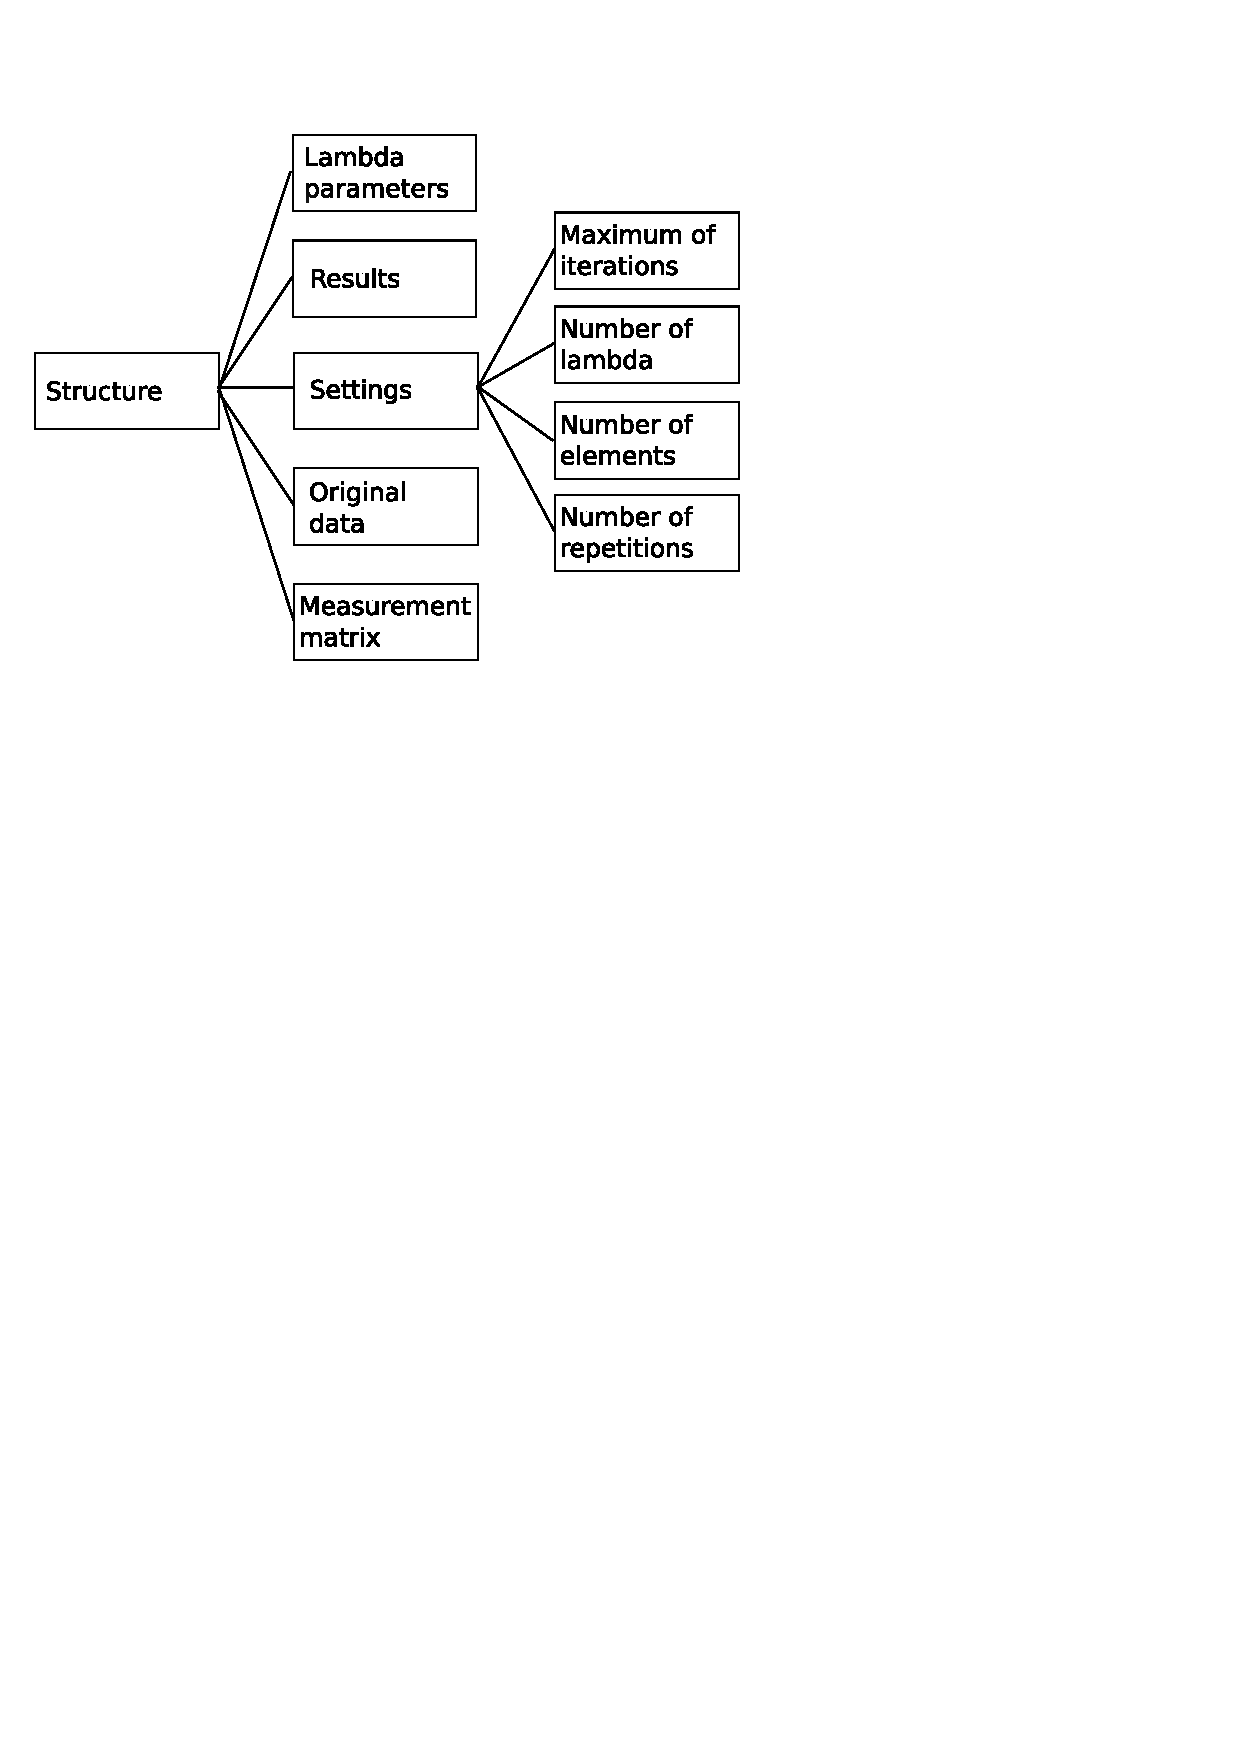
\includegraphics[scale=0.7]{obr/structure.pdf}
	\end{center}
	\caption{Struktura dat}
	\label{fig:struktura}
\end{figure}

Takto připravená struktura je již zálohována a následně také obnovována ze souboru. Pro tyto účely bylo využito funkcí \uv{save} a \uv{load}, jež jsou součástí standardní instalace prostředí MATLAB. Obě tyto funkce jsou navíc podmíněny a to tak, že v případě funkce \uv{save} je do konce simulace ukládána i dočasná iterační proměnná znázorňující aktuální počet opakování používané metody. Jak je již zřejmé, právě tato proměnná by měla být také obnovena při načítání dat. 

S takto připraveným zálohováním zbývá vytvořit jediné a to komunikaci s uživatelem. Daná komunikace byla vytvořena tak, že skript prochází umístění, kde se nachází a pokud nalezne soubor s příponou \uv{.mat}, je spolu s indexem vypsán na obrazovku a je tak vytvořeno textové menu. 

Následně uživatel volí soubor pomocí standardních vstupních zařízení, se kterým chce pracovat s uvedeným indexu. Po zvolení souboru se obnoví uložená struktura dat a pokud soubor obsahuje i iterační proměnnou, tak i ta je obnovena a to tím způsobem, že je zároveň zvýšena o $1$ a to proto, že ukládání struktury probíhá po použití algoritmu pro všechny parametry $\lambda$, nikoliv před kompletním výpočtem pro každý parametr $\lambda$. Kdyby se zmíněná proměnná neinkrementovala, tak by došlo ke zbytečnému průběhu a výpočetní čas by byl plýtván právě na tento průběh.

\begin{figure}[!ht]
	\begin{center}
		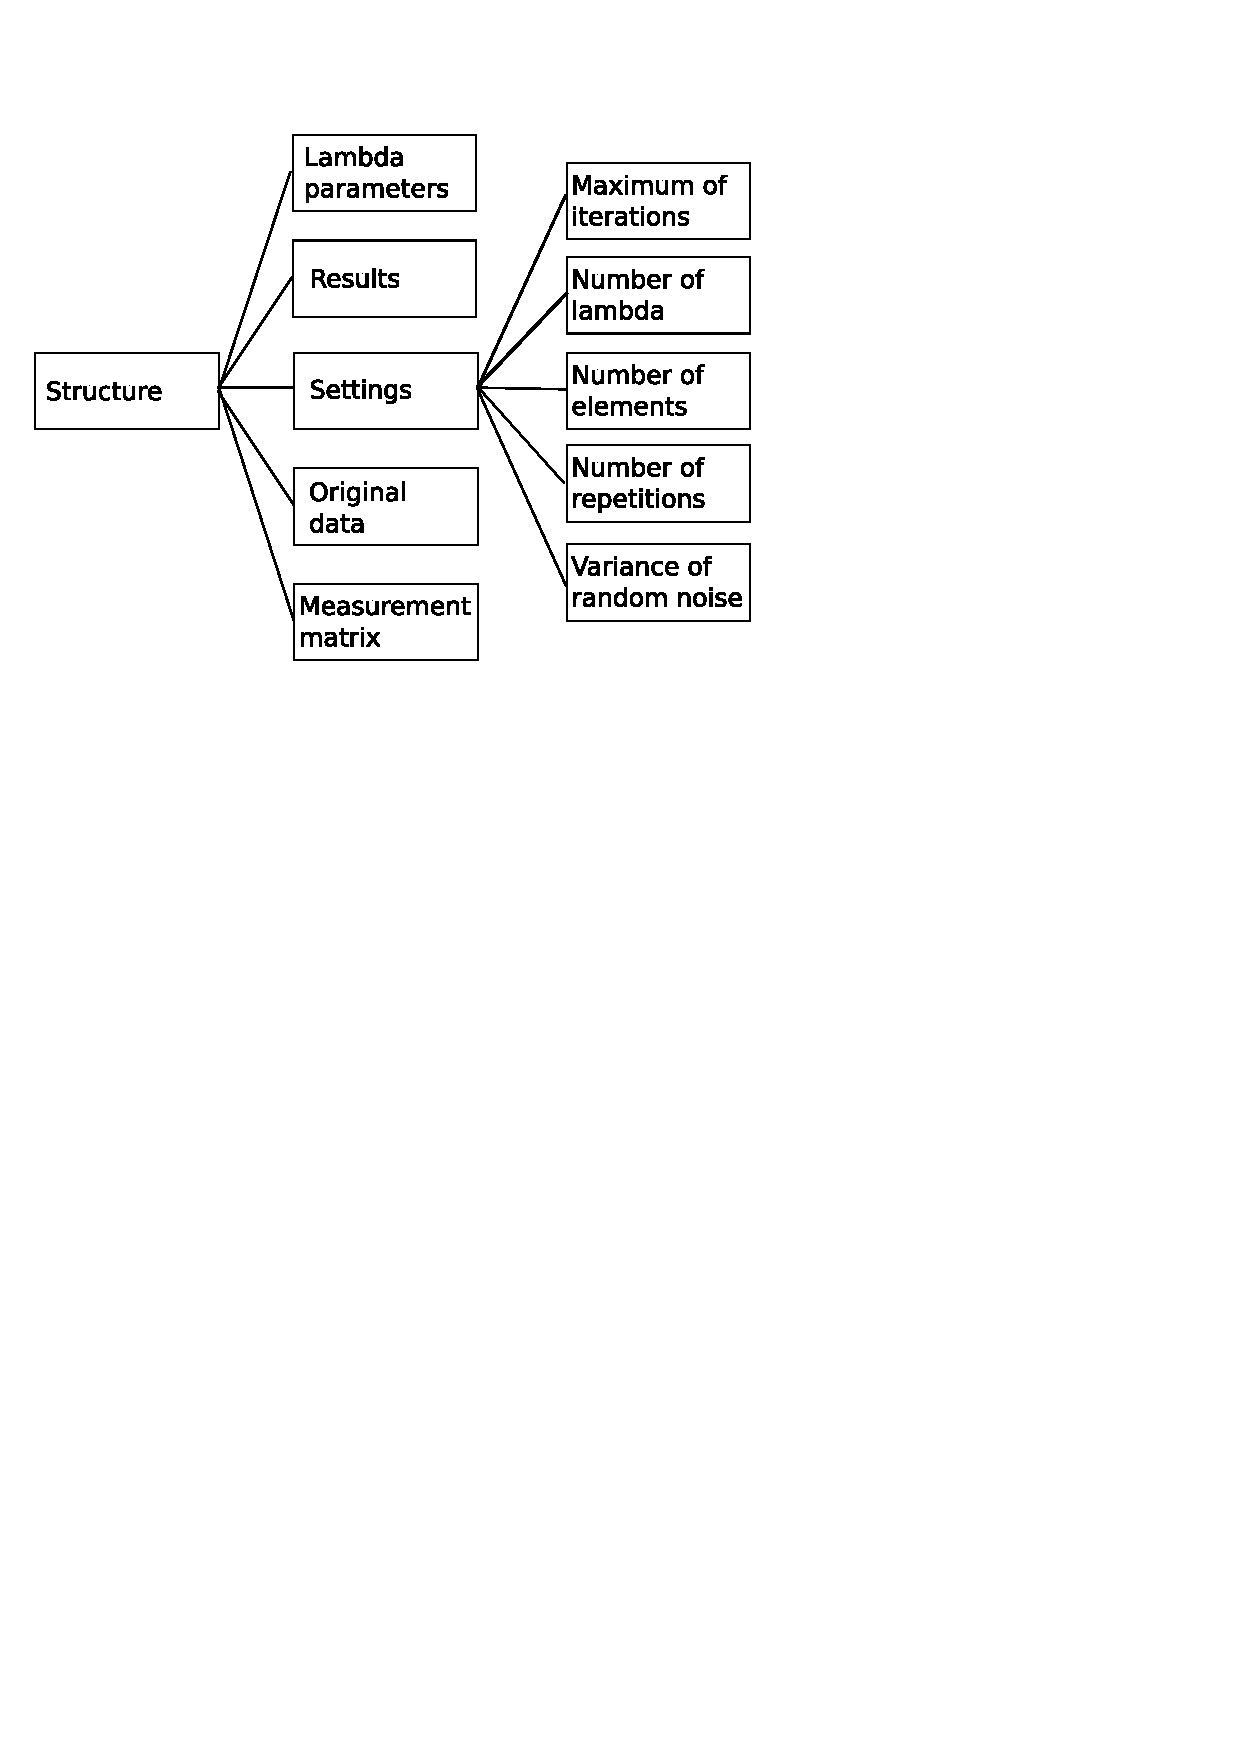
\includegraphics[scale=0.8]{obr/structure_new.pdf}
	\end{center}
	\caption{Upravená struktura pro pozdější využití}
	\label{fig:newstruct}
\end{figure}

Nicméně toto není konečná varianta. V daný moment totiž ještě nebyly zřejmé veškeré další podmínky pro vytvoření analytické předpovědi. Pro vytvoření analytické předpovědi je totiž důležitý šum v komprimovaném signálu dat, jak bude vysvětleno v další kapitole. Tento šum musí mít malý rozptyl a s takto definovanou strukturou by již nebylo možné zjistit, jaký rozptyl byl zvolen. Z předestřeného důvodu došlo k rozšíření původní struktury dat na novou, dle obrázku \ref{fig:newstruct}.

\section{Upozornění uživatele}
\label{subch:notifications}
Dalším rozšířením, které bylo realizováno, je možnost upozornění uživatele na dokončení simulace. Jednou z variant bylo využít e-mailových služeb přímo v prostředí MATLABu, nicméně toto by mělo tu nevýhodu, že by nešlo spustit současně více různých skriptů, které by využívaly e-mailové služby a posílaly tak informace o svém průběhu více uživatelům. 

Aby nebylo potřeba využívat prostředí MATLABu, byl vytvořen jednoduchý skript v jazyku Python a služby Pushbullet. Jedná se o službu, která umožňuje odesílat zprávy, případně i malé soubory, na zařízení uživatele, např. mobilní telefon. Za pomoci dokumentace a rozhraní Pushbullet byl vytvořen skript, který přijímá na vstupu argumenty pro název a tělo zprávy. Takto převzaté informace se naformátují do hlavičky POST dotazu spolu s přístupovým tokenem konkrétního uživatele. Pokud je uvedeným způsobem skript vykonán, uživatel dostane okamžitě upozornění na všechna svá zařízení a to buď pomocí mobilní aplikace, osobního počítače nebo webového prostředí. Výsledný skript, v němž uživatel vyplní svůj přístupový token, má následující podobu:

\begin{lstlisting}
def send_message(title, message):
	method = "POST"
	data = {"type": "note", "title": title, "body": message}
	handler = urllib2.HTTPHandler()
	opener = urllib2.build_opener(handler)
	url = 'https://api.pushbullet.com/v2/pushes'
	request = urllib2.Request(url, data=json.dumps(data))
	request.add_header('Content-Type', 'application/json')
	request.add_header('Access-Token', '')
	request.get_method = lambda: method
	opener.open(request)
\end{lstlisting}

Ve skriptu simulace je již tedy vytvořen samotný příkaz pomocí slučování řetězců. Takto připravený řetězec je následně předán funkci \uv{system} jako parametr. Pomocí dané dokumentace připravená metoda však nemusí být použita pouze pro upozornění uživatele na chybu, lze ji taktéž použít i pro odeslání mezivýsledků, aby se mohl uživatel rozhodnout, zda má simulace smysl či nikoliv. 

Případně lze zachytávat výjimky simulace, např.: poškozený soubor s uloženou strukturou, které nebyly patrné při běžném použití, upozornit tak včas uživatele na tuto chybu a neplýtvat časem uživatele, který by jinak čekal na konec simulace.

Dalším možným rozšířením tohoto skriptu je využít odlišných metod služby Pushbullet a docílit toho, že si uživatel bude moci zvolit pouze konkrétní zařízení, na která bude chtít zasílat upozornění z vývojového prostředí MATLAB.

\section{Výsledek pro $\left\| \cdot \right\|_{2}^{2}$ LASSO}
\label{subch:resultL22}
Se simulací, připravenou dle popisů v předchozích podkapitolách, již lze přistoupit k samotnému použití. Na začátku simulace je důležité zvolit několik parametrů: počet parametrů $\lambda$ a jejich rozsah, počet prvků původních dat $x$, počet řádků měřících matic $A$ a také počet opakování simulace. Toto nastavení je také uloženo ve struktuře, jak bylo vysvětleno v předchozí podkapitole. 

Po ukončení, často velice dlouhé simulace, je získána empirická závislost kvadratické chyby nalezeného řešení od skutečných dat pro každý prvek z vektoru parametrů $\lambda$. 

Obecně lze rozdělit parametr $\lambda$ do 3 regionů. První z nich, tzv. $R_{off}$, definující interval $\left\langle 0, \lambda_{crit}\right\rangle$, kde $\lambda_{crit}$ značí začátek postupného klesání kvadratické chyby. Obdobou je region $R_{\infty}$ s intervalem $\left\langle\lambda_{max}, \infty\right\rangle$, kde $\lambda_{max}$ udává, pro který parametr $\lambda$ je již chyba maximální možná. Poslední z regionů $R_{on}$, nejdůležitější region, vytváří interval $\left(\lambda_{crit}, \lambda_{max}\right)$. V tomto intervalu se již nachází globální minimum, tedy parametr $\lambda$, pro který je kvadratická chyba nejmenší možná.

Očekávána byla křivka s jedním globálním minimem a ostatní hodnoty získané dle parametru $\lambda$ daleko větší než je ono globální minimum a to z důvodu, velké tolerance nebo malého kroku algoritmu podle toho, do jakého regionu spadá konkrétní hodnota parametru $\lambda$. Důvody tohoto očekávání budou popsány v další kapitole \ref{ch:vysledky}. Pro ilustraci byla vytvořena simulace pro vektor dat $x$, která je shodná v obou případech. V prvním případě nebyl využit náhodný šum $z$ s malým rozptylem. V druhém případě již šum byl uvažován. Proto je možné získat většinou křivky, které jsou podobné následujícím grafům a vycházejí z uvedených podmínek:

\begin{figure}[!ht]
	\begin{center}
		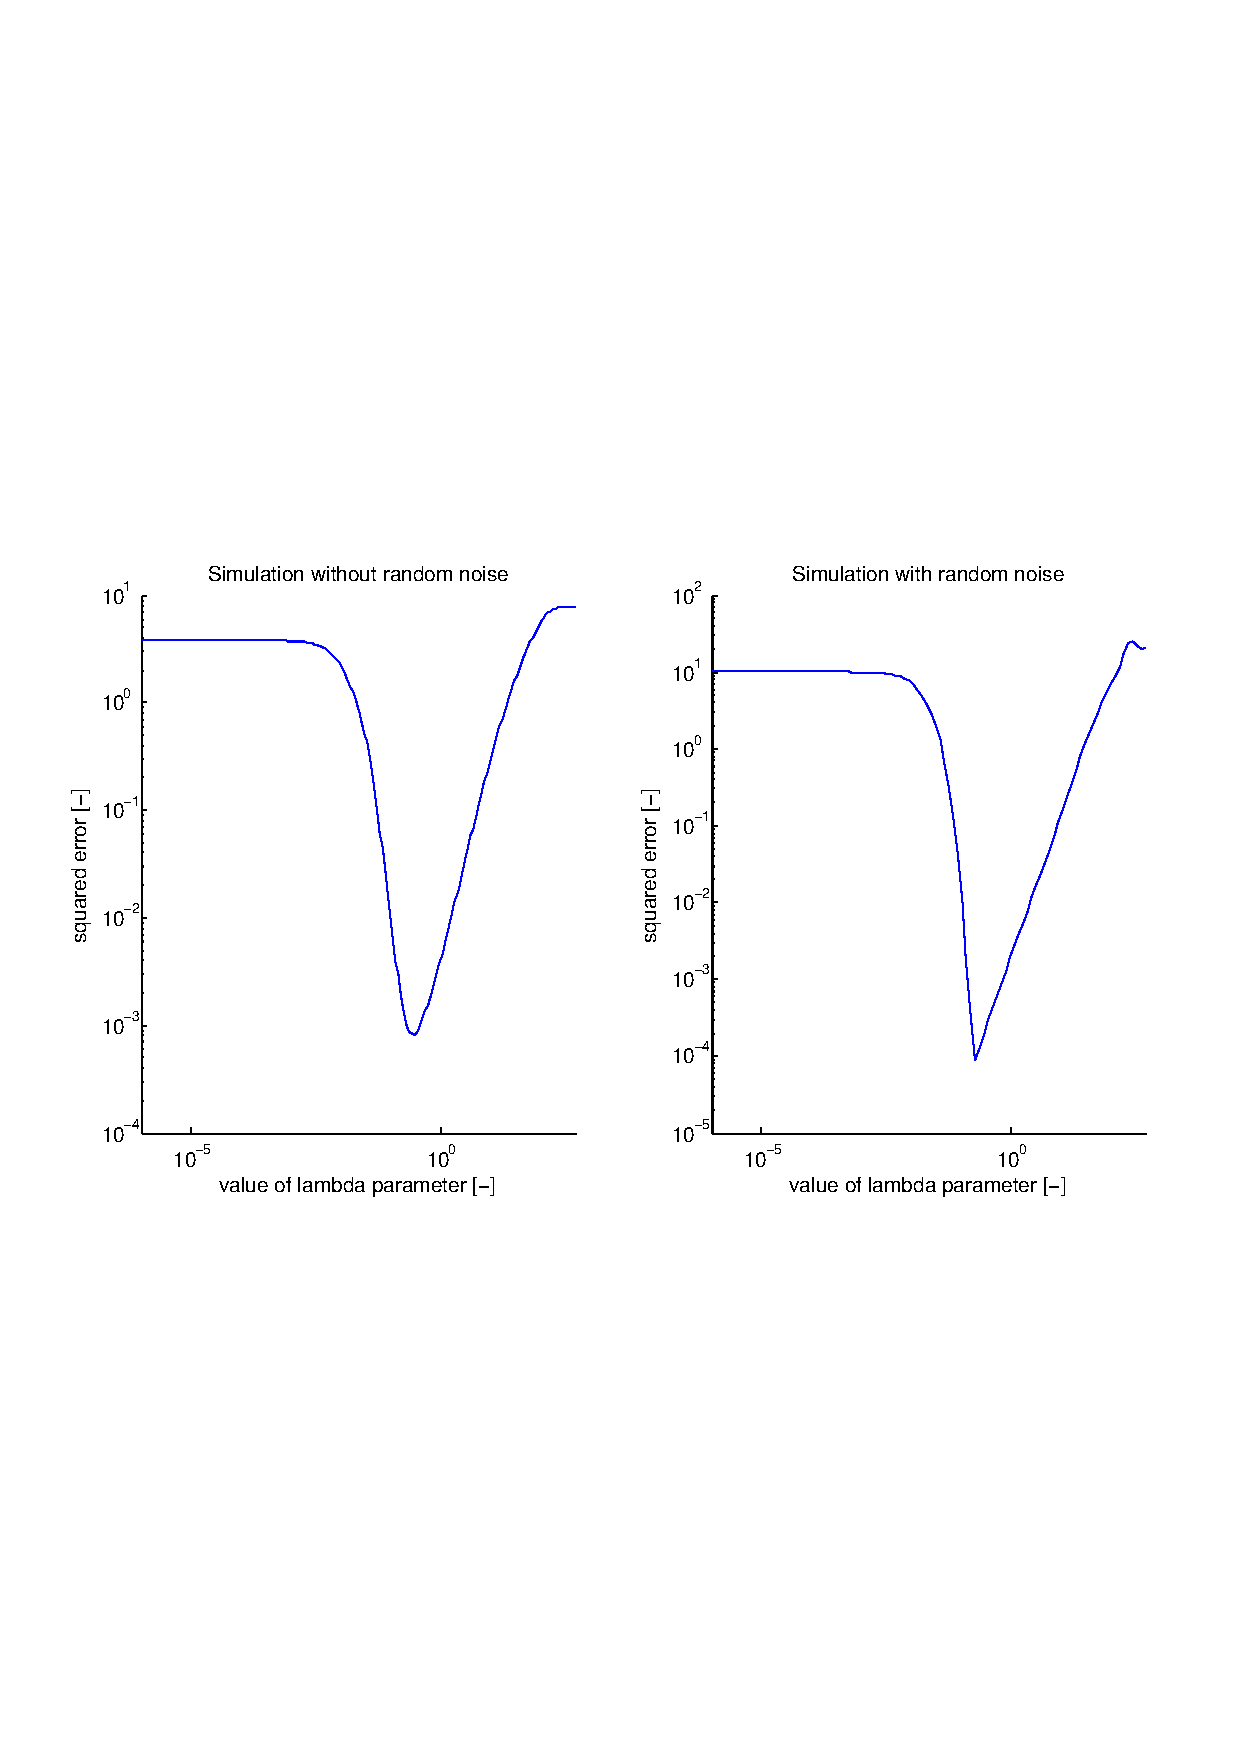
\includegraphics[scale=0.7]{obr/l22simulation.pdf}
	\end{center}
	\caption{Simulace pro $\left\| \cdot \right\|_{2}^{2}$ LASSO}
	\label{fig:l22sim}
\end{figure}

\chapter{Výsledky}
\label{ch:vysledky}
Tato kapitola se bude zabývat získáním výsledků pomocí naimplementovaných algoritmů, odvozením vzorců pro výpočet analytické chyby vybraného, ale i obdobného, problému a porovnáním takto získaných výsledků. 

Jelikož odvození vztahu pro výpočet kvadratické chyby nalezeného řešení od původních dat dle parametru $\lambda$ pro $\left\| \cdot \right\|_{2}^{2} $ LASSO je velice obtížné, je zvolen jiný přístup, který je využíván velice často pro zadaný problém i v pracích, které se zabývají uvedenou problematikou detailněji. Tento přístup využívá té vlastnosti, že lze použít jinou variantu optimalizačního problému LASSO a to $\left\| \cdot \right\|_{2}$ LASSO, pro kterou je analýza daleko jednodušeji proveditelná a následně na získanou analýzu aplikovat mapovací funkci. Nicméně toto nás vrací zpět na začátek zadání. Jednotlivé kroky takto definovaného přístupu budou popsány, pro přehlednost, v jednotlivých podkapitolách.

\section{Rekonstrukce dat s využitím proximálního algoritmu}
\label{subch:l2Prox} 
Velice důležitým prvním krokem je samotná rekonstrukce dat. Jelikož již byl implementován proximální algoritmus řešící obdobnou úlohu, je také využit jako první volba. Protože je algoritmus vhodně rozčleněn do bloků, změna je velice jednoduchá a spočívá ve změně gradientu funkce z kapitoly \ref{ch:fwbw} na: 

\begin{equation} \label{eq:l2Grad}  \tag{Vzorec \theVzorce}
\partial f(x) = -A^{T} \cdot \frac{\left(y-A \cdot x\right)}{\left\| y - A \cdot x\right\|_{2} }
\end{equation}
\myequations{\ref{eq:l2Grad} - Gradient $\left\| \cdot \right\|_{2}$ LASSO}
\stepcounter{Vzorce}

Protože pro tento problém nemusí platit, a také neplatí, podmínky optimality, byly právě zmíněné funkce, realizující takto definované zastavující kritérium, odebrány. Je vhodné připomenout, že podmínky optimality jsou definovány pouze pro $\left\| \cdot \right\|_{2}^{2} $ LASSO. Následně byl proveden první test funkčnosti. Jako prvotní nastavení bylo zvolen parametr znázorňující maximální počet iterací a to v hodnotě 3000. Jelikož výsledek nebyl přijatelný, viz následující graf, proběhla podrobnější analýza chování.

\begin{figure}[!ht]
	\begin{center}
		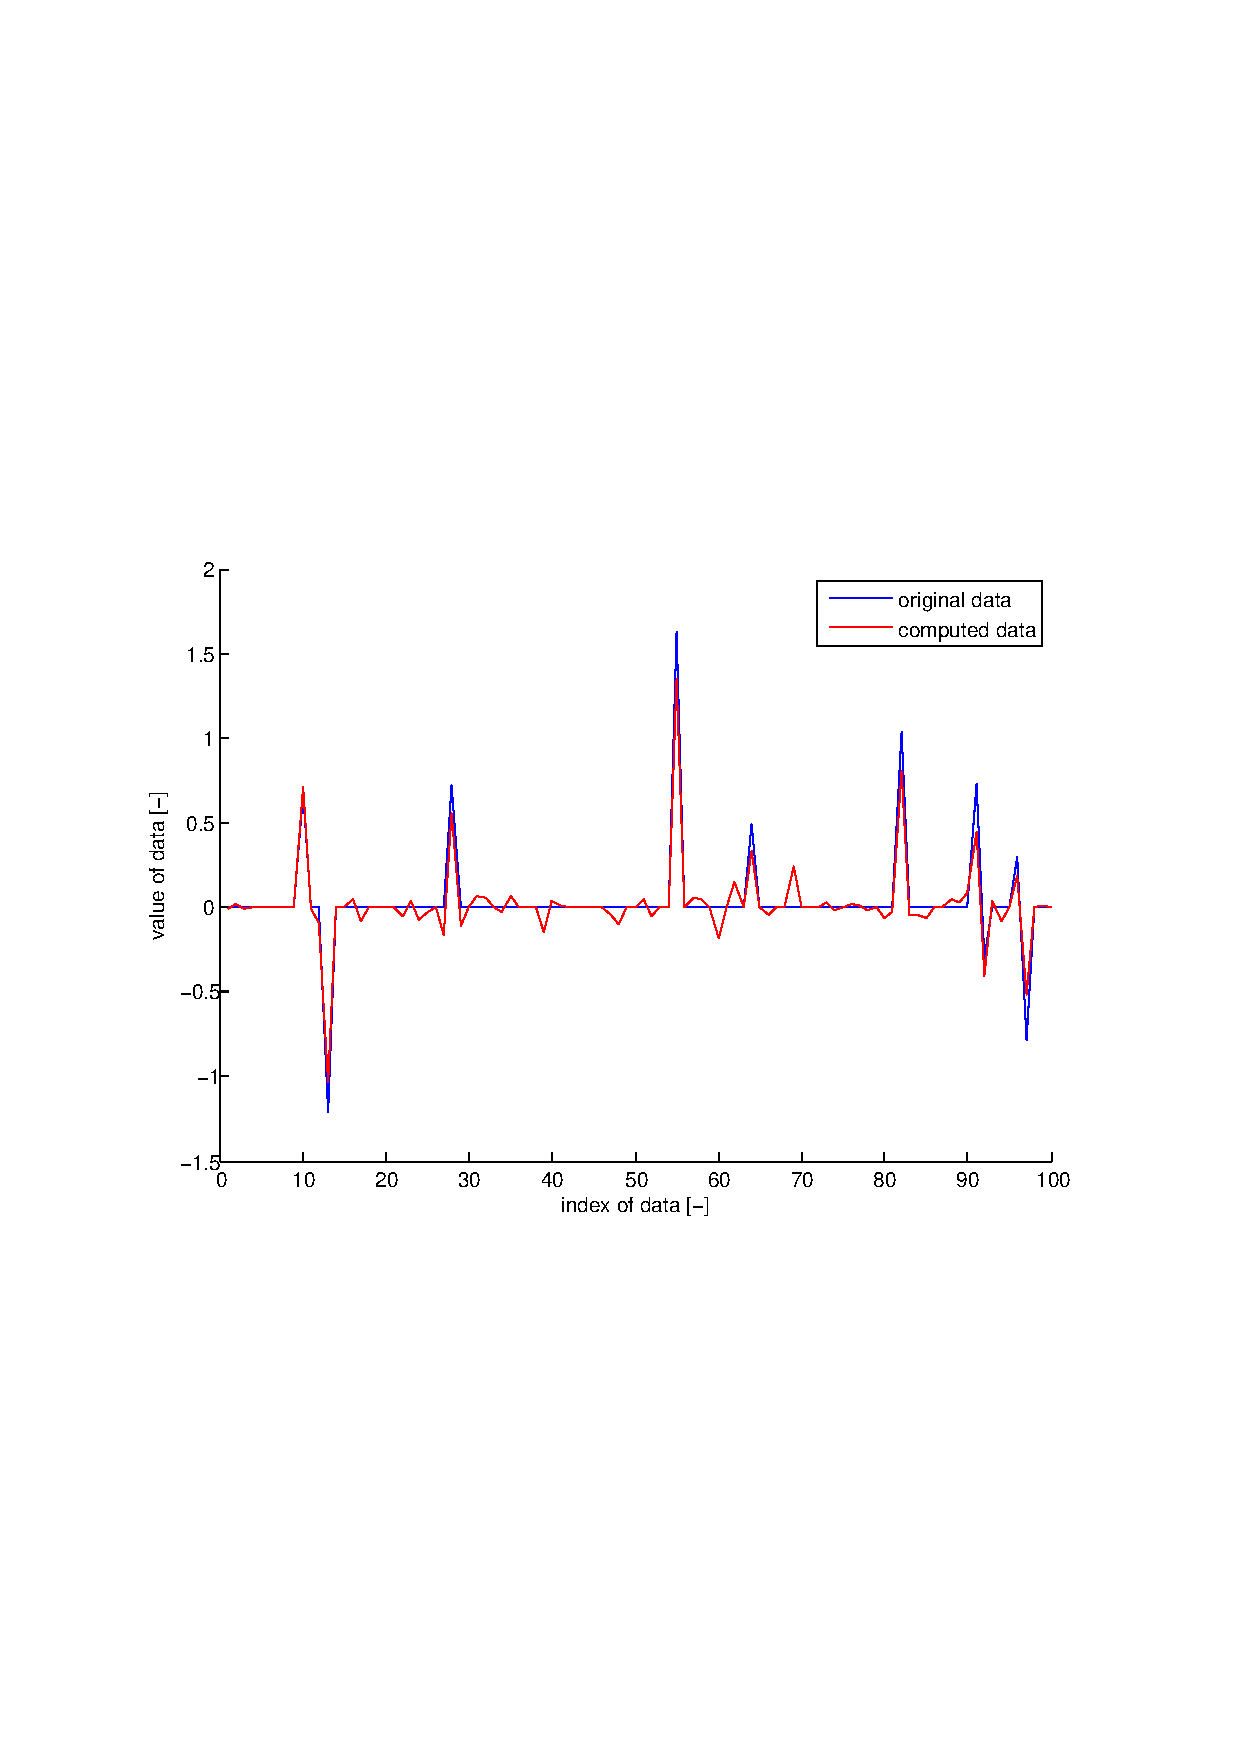
\includegraphics[scale=0.7]{obr/l2-firsttry.pdf}
	\end{center}
	\caption{První experiment s $\left\| \cdot \right\|_{2}$ LASSO}
	\label{fig:l2first}
\end{figure}

Z průběhu algoritmu vyplynulo, že se varianta daného algoritmu velice liší od původní verze. Předložená verze algoritmu nekonverguje přímo k řešení, ale kmitá ke správnému výsledku a to se stále se zmenšující intenzitou a tedy některé iterace algoritmu jsou zbytečné. Z nastalého pozorování vyšlo najevo, že algoritmus je výrazně pomalejší a je nutné zvolit větší počet iterací než dosud. Pro nový experiment bylo nastaveno maximální počet 10000 průběhů algoritmu a byl tak získán nový graf rekonstrukce vektoru dat:

\begin{figure}[!ht]
	\begin{center}
		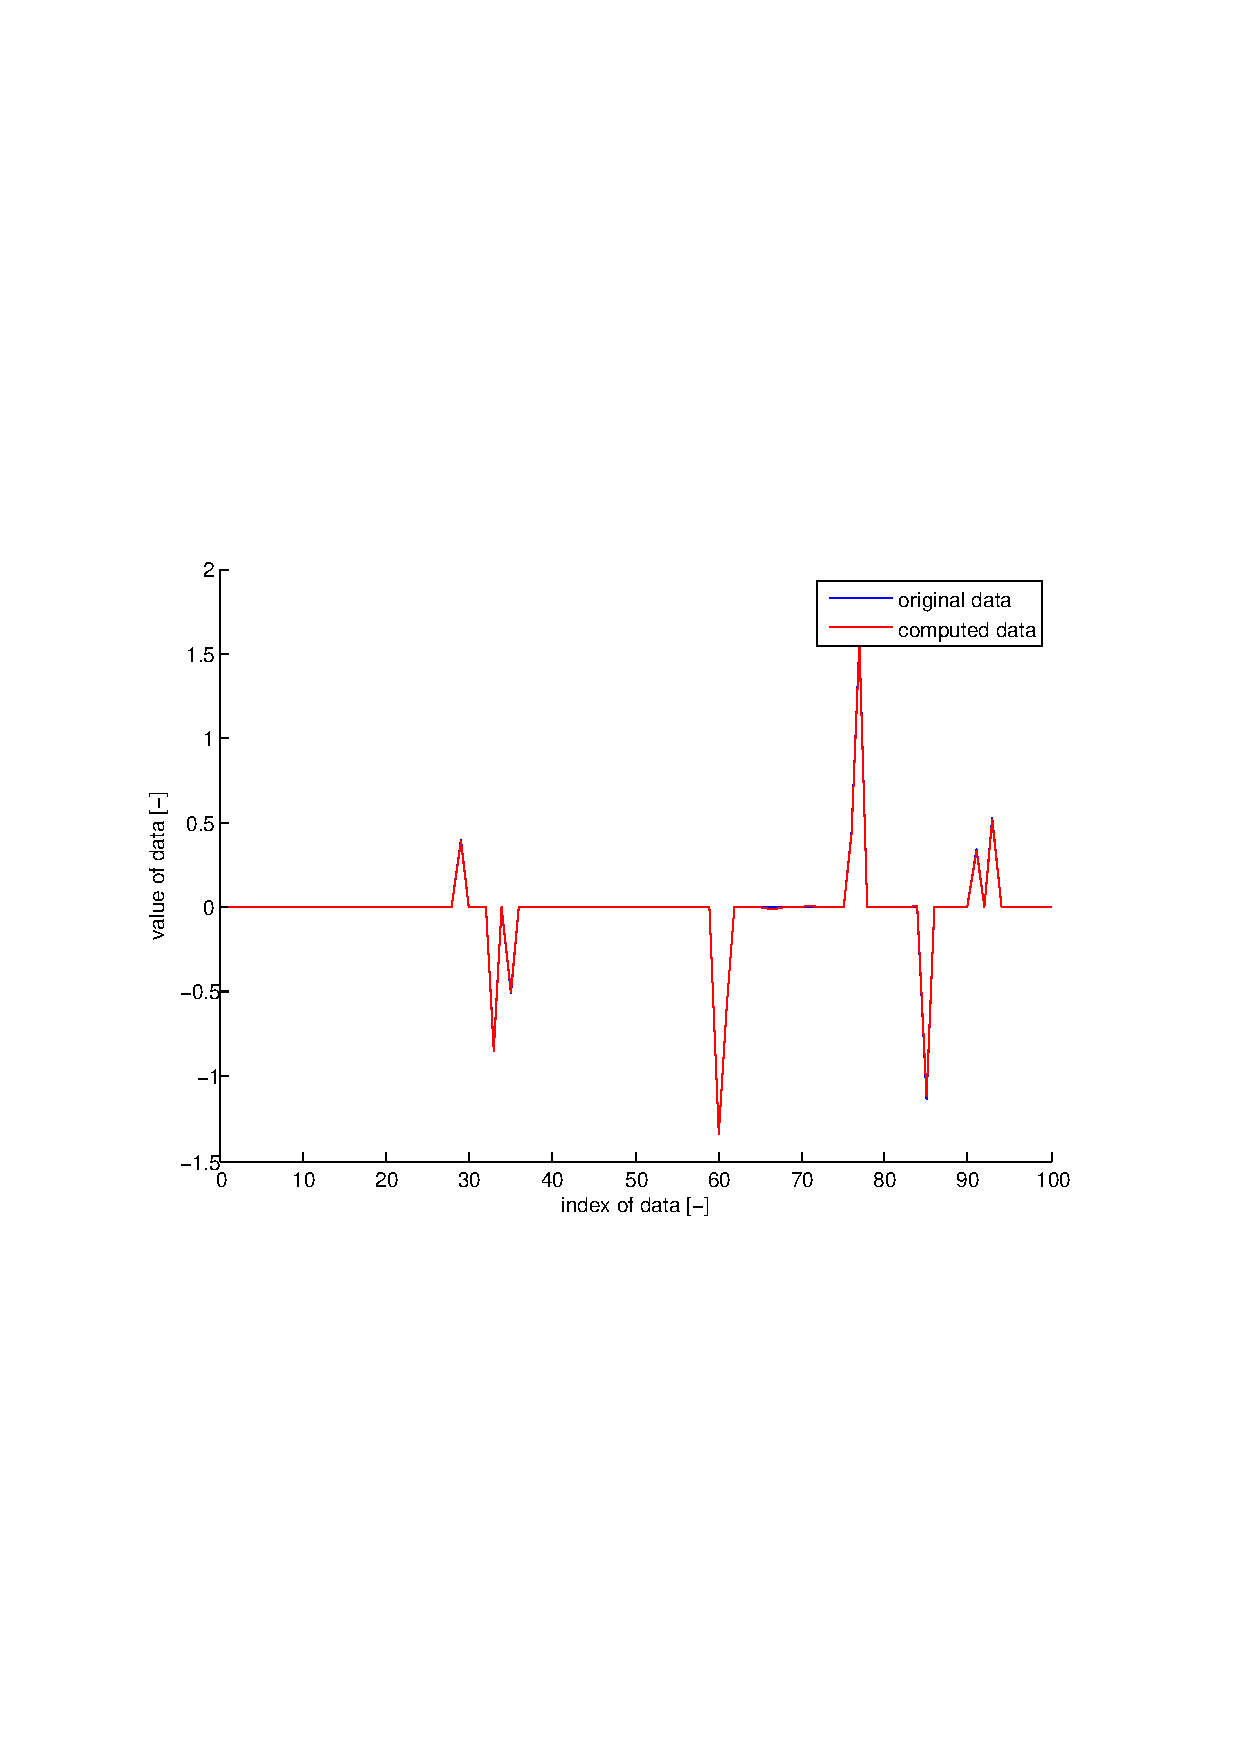
\includegraphics[scale=0.7]{obr/l2-finish.pdf}
	\end{center}
	\caption{Druhý experiment s $\left\| \cdot \right\|_{2}$ LASSO}
	\label{fig:l2finish}
\end{figure}

\section{Rekonstrukce dat pomocí CVX knihoven}
\label{subch:l2CVX}
Jelikož i samotný gradient předchozího algoritmu funkce je velice náročný na výpočet a nelze si tudíž předpřipravit před samotným prováděním algoritmu žádné pomocné proměnné, viz \ref{eq:l2Grad}, bylo využito open source knihoven CVX. Tyto knihovny jsou primárně zaměřené na modelování konvexních optimalizací a tak využívají daleko přesnějších a rychlejších algoritmů, než bylo použito v předkládané bakalářské práci. 

Po přidání zmíněného balíku do vývojového prostředí MATLAB lze použít modelovacího jazyka pro vytvoření jednoduchého skriptu, jenž bude provádět totéž, co bylo dosud implementováno. Jelikož se jedná o snadno použitelný modelovací jazyk, není náročné implementovat skript, který bude minimalizovat vybraný problém a může vypadat následovně: 

\newpage

\begin{lstlisting}
y = A*x + sum;
cvx_begin quiet
variable x_n(pocet_prvku)
minimize((norm(y-A*x_n,2)+lambda(j)*norm(x_n,1)))
cvx_end
\end{lstlisting}

Jak je vidět, tak balík knihoven CVX opravdu velice výrazně zjednodušuje realizaci vybraného problému. Vše je uvedeno příkazem \uv{cvx\_begin}, jímž začínají deklarace proměnných a funkcí, spolu s parametrem \uv{quiet}. Zmíněný příkaz je nastaven právě takto, aby byl potlačen výpis částečných výsledků během opakování této části skriptu. Následně je deklarována proměnná $x_n$, přes kterou se minimalizuje zadaný problém a to o předem daném počtu prvků. Poté se již používá příkaz \uv{minimize}, kterému se deklaruje funkce, již chceme minimalizovat. V této funkci se využívá standardní funkce \uv{norm} a to jak pro zápis $\left\| y - A \cdot x_n\right\|_2$, tak pro $ \left\| x \right\|_1  $, která je ještě zvětšena, resp. zmenšena, prvkem z vektoru parametrů $\lambda$ s indexem $j$. Vše je uzavřeno druhou polovinou párového příkazu a to příkazem \uv{cvx\_end}. Po skončení průběhu skriptu získáme následující graf \ref{fig:cvx}.

\begin{figure}[!ht]
	\begin{center}
		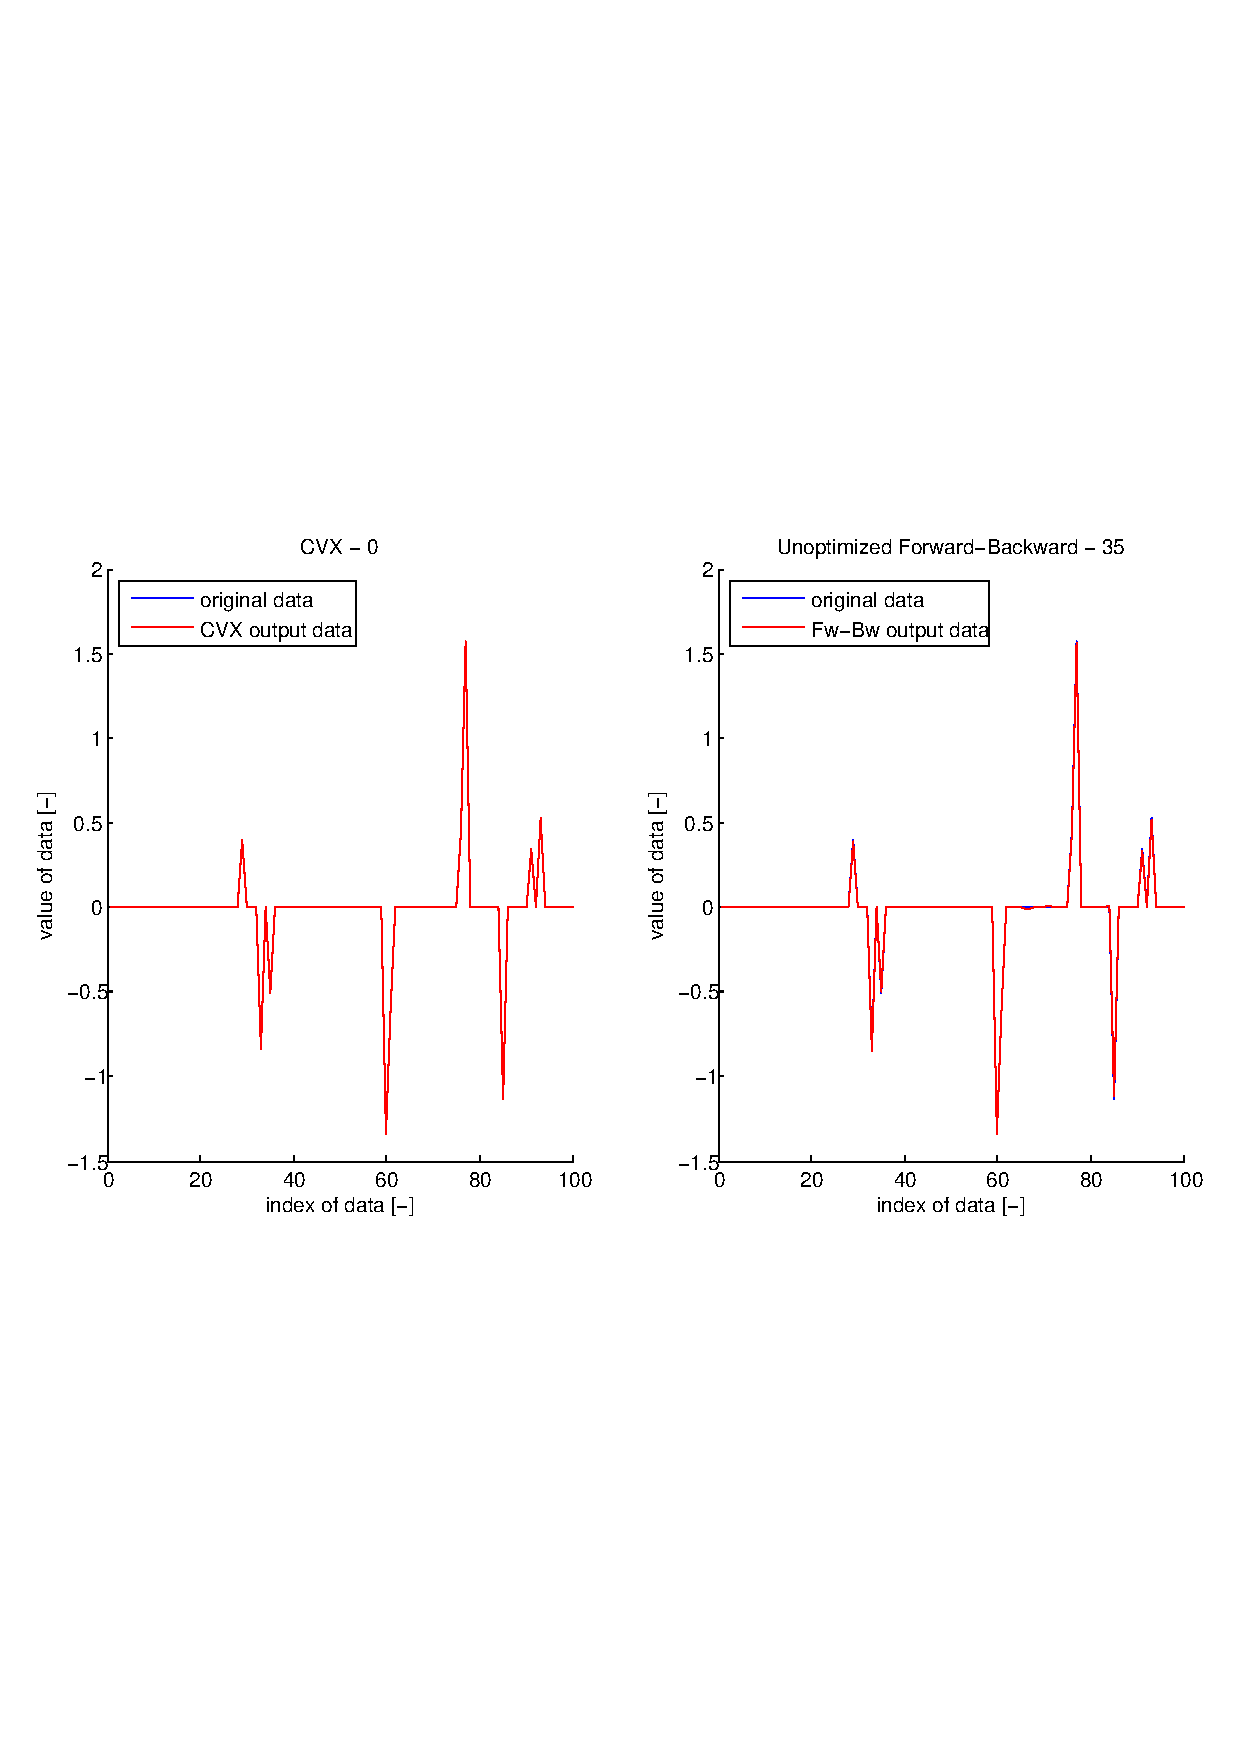
\includegraphics[scale=0.7]{obr/cvxvsprox.pdf}
	\end{center}
	\caption{Porovnání CVX výsledku s proximálním algoritmem}
	\label{fig:cvx}
\end{figure} 

Na první pohled se jedná o prakticky totožná data. Nicméně při podrobnějším zkoumání, bylo zjištěno, že žádný z prvků nezkonvergoval k úplně správné hodnotě a to ani pro nulové prvky. K odstranění popsaných nedostatků by tedy bylo nutné vytvořit další blok kódu, který by uvedené nedostatky odstraňoval. 

Pro porovnání bylo využito také dopředno-zpětného algoritmu z této kapitoly. Pro verzi algoritmu upravenou dle \ref{subch:l2Prox} nejsou výsledky optimální, jako v případě $\left\| \cdot \right\| _{2}^{2}$ LASSO problému, nicméně algoritmus úspěšně zkonvergoval ke správným hodnotám ve 35 případech ze 100.

\section{Analytická předpověď pro $\left\| \cdot \right\|_{2}$ LASSO}
\label{subch:l2Analytic}
Nicméně, tyto kroky jsou opět pouhým empirickým pozorováním a stále to neříká nic o závislosti kvadratické chyby nalezeného řešení od správného na parametru $\lambda$. Z tohoto důvodu tedy musí být sestavena první ze simulací, která bude realizovat analytickou předpověď.

Jednou z možností, jak vytvořit analytickou předpověď, je využít kvadratického programování, tj. příkazu \uv{quadprog}, ve standardní instalaci MATLABu a to na funkci:

\begin{equation} \label{eq:analyza}  \tag{Vzorec \theVzorce}
\underset{s \in \partial f(x_0)} {\mathrm{min}} ~\left\{ \left\| h - \lambda \cdot s\right\| ^2 \right\}
\end{equation}
\myequations{\ref{eq:analyza} - Funkce pro vytvoření analytické předpovědi}
\stepcounter{Vzorce}

V této funkci dochází k minimalizaci celkové hodnoty přes subdiferenciál funkce $\left\| x\right\|_1 $. Jak již bylo připomenuto v kapitole \ref{ch:optproblem}, tato funkce nemá vlastní derivaci a tudíž musí být využit jiný přístup. Transformovat danou funkci na skalární součin $s \cdot x^{T}$, který již lze derivovat. Popis subdiferenciálu pro zmíněnou funkci je následující:

\begin{equation} \label{eq:subdif} \tag{Vzorec \theVzorce}
s = \begin{cases}
s_i = 1 & i \in s_+(x_0)\\
s_j = -1 & j \in s_-(x_0)\\
-1 \le s_k \le 1 & k \in s_0(x_0)
\end{cases}
\end{equation}
\myequations{\ref{eq:subdif} - Subdiferenciál $\left\| \cdot \right\|  _1$}
\stepcounter{Vzorce}

Výše zmíněná struktura rozděluje vektor $s$ na tři části a to na: kladnou část, zápornou část a nulovou část, proto je využito spodních indexů \uv{+}, \uv{-} a \uv{0} u označení jednotlivých částí. 

S takto definovanými funkcemi již lze přistoupit k samotné implementaci. Jak již bylo řečeno, využije se příkazu \uv{quadprog} a musí být tedy původní funkce analýzy upravena do příkazem definovaného stavu. Po patřičných úpravách je tak získán tvar:

\begin{equation} \label{eq:quad} \tag{Vzorec \theVzorce}
\begin{split}
\left\| h - \lambda \cdot s\right\|_{2}^{2}  & = \frac{1}{2} \cdot 2 \cdot \lambda^{2} \cdot s^{T} \cdot I \cdot s - 2 \cdot \lambda \cdot h^{T} \cdot s\\
H & = 2 \cdot \lambda^{2} \cdot s^{T} \cdot I\\
f & = - 2 \cdot \lambda \cdot h^{T}
\end{split}
\end{equation}
\myequations{\ref{eq:quad} - Proměnné analytické předpovědi pro kvadratické programování}
\stepcounter{Vzorce}

S připravenými proměnnými $H$ a $f$ již je možné použít příkaz \uv{quadprog}. Nicméně, jelikož subdiferenciál je definován pouze pro hodnoty $[-1, 1]$, je nutné využít také omezující podmínky tohoto příkazu a to dle \ref{eq:subdif}. Poté se již provede Monte Carlo simulace na zhotoveném algoritmu a průměr dílčích výsledků poskytuje analytickou předpověď. 

\section{Aplikace Monte Carlo simulace na minimalizace}
\label{subch:l2Sim}
Velice důležitým prvním krokem je, využít již zhotovené analytické předpovědi a použít proměnné, které se nesmí změnit, mezi které patří: parametry $\lambda$ a vstupní vektor dat $x$. S připravenými proměnnými již je možné realizovat jednotlivé simulace. Jelikož hlavní téma této bakalářské práce jsou proximální algoritmy, bude se jimi také začínat.

Pro verzi simulace s využitím proximálního algoritmu je realizace velmi jednoduchá. Jelikož již byla tato simulace realizována, viz \ref{ch:simulace}, a zároveň byla navržena tak, aby ji šlo jednoduše modifikovat, stačilo pouze použít nový skript, řešící $\left\| \cdot \right\|_{2} $ LASSO, a dosadit ho na patřičné místo ve skriptu simulace. Kvůli většímu množství iterací však tato simulace probíhá velmi dlouhou dobu, v nejhorších případech pro 1000 opakování a 100 parametrů $\lambda$ trvá průběh minimálně tři dny.

Jelikož druhá varianta využívá knihoven CVX, nešlo takto jednoduše modifikovat danou simulaci a musela tedy být vytvořena nově. Bylo využito stejného popisu jako v kapitole \ref{ch:simulace} a tedy výsledná podoba skriptu, provádějící tuto simulaci má následující podobu: 

\begin{lstlisting}
for i = 1:pocet_opakovani
	y = A*x + sum;
	for j = 1:pocet_lambda
		cvx_begin quiet
		variable x_n(pocet_prvku)
		minimize((norm(y-A*x_n,2)+lambda(j)*norm(x_n,1)))
		cvx_end
	end
end
\end{lstlisting}
Pro takto definované simulace získáme grafy z obrázku \ref{fig:sims}.

\begin{figure}[!ht]
	\begin{center}
		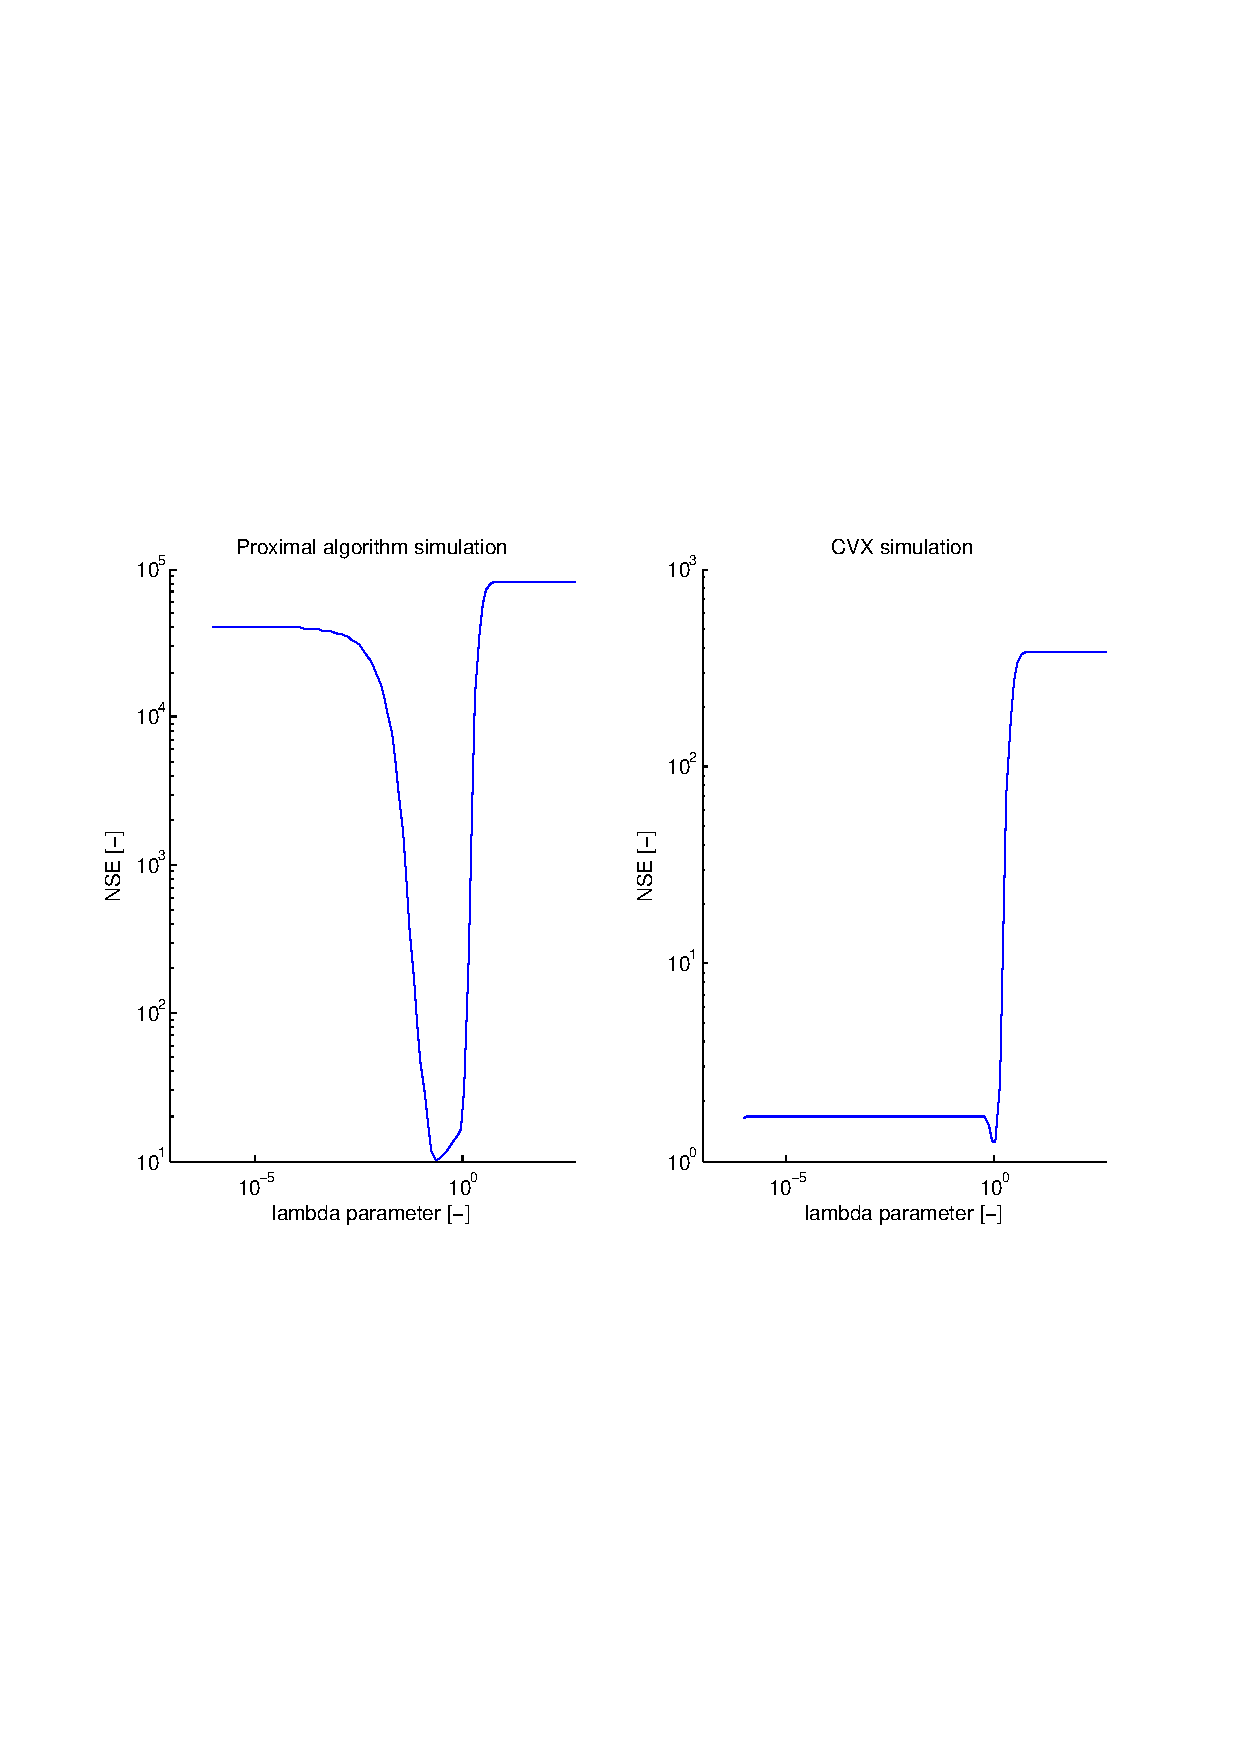
\includegraphics[scale=0.7]{obr/sims.pdf}
	\end{center}
	\caption{Porovnání simulací}
	\label{fig:sims}
\end{figure}

Je vidět, že grafy jsou odlišné a to z toho důvodu, jenž byl naznačen v \ref{subch:l2Prox}. Proximální algoritmus je výrazně pomalejší pro $\left\| \cdot \right\| _{2}$ LASSO než pro zadaný problém, tedy $\left\| \cdot \right\|_{2}^{2} $ LASSO. Ze zjištěných poznatků tedy vyplývá, že velice důležitým aspektem algoritmu je právě maximální počet iterací. 

Při bližším analyzování bylo zjištěno, že pro velmi malé parametry $\lambda$ algoritmus nezkovergoval ke správnému řešení. Příčiny jsou hned dvě. První z nich je výpočet dynamické délky kroku z kapitoly \ref{ch:fwbw}. Jelikož je délka kroku také použita v proximálním operátoru, nastane i zde problém. Funkce, která vypočítává délku kroku vrací výsledek v tisícinách. Následně je tato hodnota v proximálním operátoru, do kterého vstupuje, vynásobena parametrem $\lambda$ v řádech miliontin, vznikne tak velice malé číslo na, resp. za, přesností datového typu. S takto získaným parametrem je následně proveden výpočet a změna je téměř nulová.

Poté se tedy vypočte normalizované chyba, dle \ref{eq:NSE}. Následně je chyba vydělena rozptylem $\sigma$ náhodného šumu $z$, se kterým se pracuje v celé bakalářské práci. Jelikož algoritmus nezkonverguje ke správnému řešení, vzniká vysoká chyba, která je následně ještě více zvýrazněna tímto parametrem.

\begin{equation} \label{eq:NSE}  \tag{Vzorec \theVzorce}
NSE = \frac{\left\| y - A \cdot x\right\|_{2}^{2} }{\sigma}
\end{equation}
\myequations{\ref{eq:NSE} - Normalizovaná chyba nalezeného řešení od správného}
\stepcounter{Vzorce}

Jednou z možných variant, jak tuto chybu podstatně zmenšit, je předpověď nultého kroku algoritmu, tedy proměnné $x_{n}$. Zatím se vždy používal vektor nul a v případě prvotního odhadu by se tak chyba velice redukovala. Nicméně, zadáním této práce není vytvoření dokonalého algoritmu, který by řešil zadanou úlohu, ale vytvoření nástroje, s jehož pomocí lze pozorovat závislost kvadratické chyby nalezeného řešení od korektních dat na parametru $\lambda$ a proto toto nebylo realizováno a jedná se tak o nastínění další z možných cest, jak využít tuto bakalářskou práci v dalším výzkumu.

Z důvodu zmíněného výše tedy bude v následujících krocích použita analytická předpověď získaná za pomoci knihoven CVX, jenž je daleko přesnější než předpověď získaná pomocí proximálního algoritmu a tudíž je vhodnější pro další zpracování. 

Pro prvotní otestování byla Monte Carlo simulace spuštěna bez dalších optimalizací. Graf této simulaci lze vidět na následujícím obrázku:

\begin{figure}[!ht]
	\begin{center}
		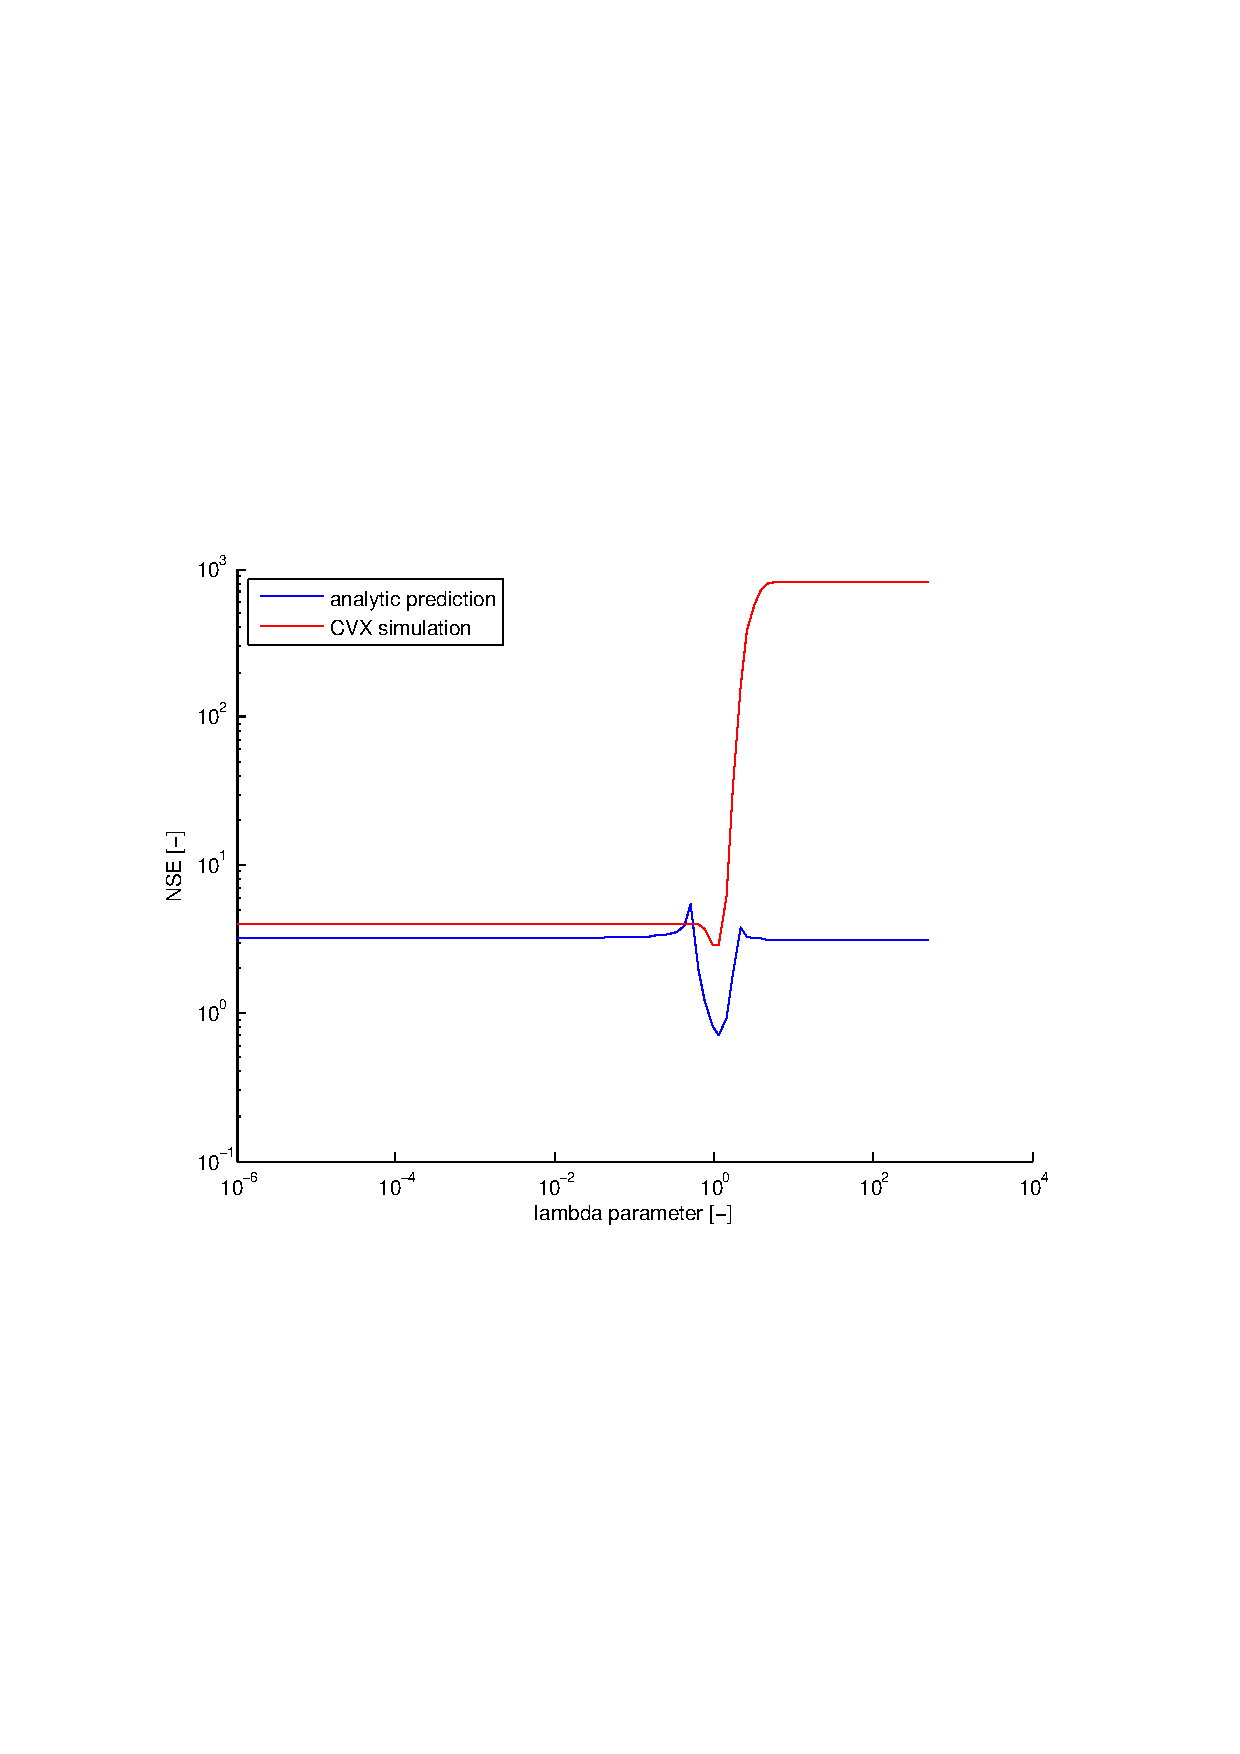
\includegraphics[scale=0.7]{obr/analytic.pdf}
	\end{center}
	\caption{Porovnání analytické předpovědi s výsledkem Monte Carlo simulace}
	\label{fig:analytic}
\end{figure}

Funkce pro vykreslení analytické křivky, dle článku \cite{hassibiClanek}, má následující předpis:

\begin{equation} \label{eq:analytic}  \tag{Vzorec \theVzorce}
f(a) : \log \frac{a}{n - a}
\end{equation}
\myequations{\ref{eq:analytic} - Funkce pro vykreslení analytické křivky}
\stepcounter{Vzorce}

V této funkci se vstupní data $a$, tedy analytická předpověď získaná v jedné z předchozích podkapitol, dělí rozdílem $(n-a)$, kde $n$ je počet řádků v měřící matici. Dále se získaný vektor normalizuje a to pomocí funkce $\log$. Jelikož však mohou nastat případy, kdy $n < a$, je důležité zmínit, že tato analytická křivka by se měla skládat ze 3 různých funkcích pro tzv. regiony zájmu. Jelikož je nejdůležitější oblastí zájmu region, kde je ono hledané minimum, nebyly ostatní regiony nadále uvažovány. 

Jak lze vidět z grafu, minimum simulace je skutečně na shodném místě s minimem analýzy. Hodnota minima je však daleko větší než u analytické předpovědi. Vzhledem k tomu, že tento krok bakalářské práce je řešen spíše formou rešerše, není tato simulace odladěna do nejmenších detailů.

\section{Aplikování mapovací funkce na analytickou předpověď  $\left\| \cdot \right\| _{2}$ LASSO}
\label{subch:mapFunc}
Vzhledem k tomu, že jsou v této práci zmíněny 2 funkce využívající parametry $\lambda$, je důležité je důsledně odlišovat a to pro každou variantu zadaného problému. Proto bude nadále používán parametr $\tau$ pro $\left\| \cdot \right\|_{2}^{2} $ LASSO a pro $\left\| \cdot \right\|_{2} $ LASSO bude parametr $\lambda$ zachován. V obecných případech neplatí, že $\tau = \lambda$ a proto musí být použita funkce, konkrétně mapovací funkce, která převede původní parametry $\lambda$, které byly využity pro vytvoření analytické předpovědi, na nové parametry $\tau$, které se použijí pro výpočet empirického pozorování v Monte Carlo simulaci.
Protože je tato práce založena na článku \cite{hassibiClanek}, bylo také využito mapovací funkce, která je zde použita. Předpis této funkce je následující:

\begin{equation} \label{eq:map}  \tag{Vzorec \theVzorce}
\tau = \lambda \cdot NSE
\end{equation}
\myequations{\ref{eq:map} - Mapovací funkce}
\stepcounter{Vzorce}

V tomto vzorci se tedy původní parametry $\lambda$ násobí s normalizovanou chybou analytické předpovědi, jejíž předpis je znázorněn v předchozí podkapitole, viz \ref{eq:NSE}. S novými parametry $\tau$ je možné přejít k výpočtu numerické simulace pro $\left\| \cdot \right\|_{2}^{2} $ LASSO a pozorovat tak závislost kvadratické chyby nalezeného řešení od původních dat na novém parametru $\tau$.

\chapter{Závěr}
\label{ch:end}
Jak je patrné z celé bakalářské práce, je toto téma velice rozsáhlé a nebylo možné zde popsat jednotlivé kroky do větších detailů, jelikož se využívá složitých matematických postupů. Právě kvůli těmto matematickým základům zůstaly simulace spíše v rešerším stádiu. Je tak možné využít tuto bakalářskou práci pro další studie a vytvořit tak odpovídající simulace, které budou daleko přesnější než rešeršní verze, které byly doposud využívány. Nicméně při zběžném porovnání výsledků numerických simulací s těmi, které byly uvedeny v hlavním zdroji této práce, tj. \cite{hassibiClanek} a \cite{hassibiPrednaska}, jsou dílčí výsledky podobné svým průběhem těm, které byly předpokládány na základě doporučených studijních materiálů.

Z celé technické dokumentace je tedy vidět, že bylo vytvořeno hned několik nástrojů. Prvním z nich je samotný proximální algoritmus a příslušející proximální operátor. Díky výhodné implementaci je možné ho dále rozšiřovat o další bloky, zajišťující lepší výsledky nebo využít tento základní algoritmus i pro jiné účely než byly zmíněny v této bakalářské práci. 

Poté byla implementována rešerší verze metody Monte Carlo. Ta se stará o provedení algoritmu na větším množství dat. Vhodnou implementací se docílilo toho, že výsledky nelze ztratit během zdlouhavého výpočtu a zároveň je uživatel upozorněn na různé události, např. konec simulace.

V průběhu této bakalářské práce byly také naznačeny další způsoby, jak by se nechal v tomto studijním tématu postupovat dál, např. neřešit vše ve vývojovém prostředí a jazyce MATLAB, ale využít jiné programovací jazyky, případně jejich nadstavby, a vhodnou paralelizací výrazně zrychlit celkové výpočty. 

Získané poznatky se shodovaly s dlouholetou prací Babaka Hassibiho, Ph.D. z California Institute of Technology, jehož výzkum byl základem předkládané práce.

\renewcommand{\bibname}{Literatura}
\begin{thebibliography}{99}
\bibitem{homotopy}KOLDOVSKÝ, Zbyněk a TICHAVSKÝ, Petr, "A Homotopy Recursive-in-Model-Order Algorithm for Weighted Lasso," Proc. of the 41st IEEE International Conference on Audio, Speech, and Signal Processing (ICASSP 2014), Florence, Italy, pp. 4151-4155, May 2014.
\bibitem{hassibiPrednaska}HASSIBI, Babak. Recovering Structured Signals in Noise: Comparison Lemmas and the Performance of Convex Relaxation Methods [online]. California Institute of Technology, 2015 [cit. 2016-05-04]. Dostupné z: $www.eusipco2015.org/files/EUSIPCO2015\_TUTO3.pdf$
\bibitem{hassibiClanek}OYMAK, Samet; THRAMPOULIDIS, Christos; HASSIBI, Babak. The squared-error of generalized LASSO: A precise analysis. In: Communication, Control, and Computing (Allerton), 2013 51st Annual Allerton Conference on. IEEE, 2013. p. 1002-1009.
\bibitem{proxAlg1}PARIKH, Neal; BOYD, Stephen P. Proximal Algorithms. Foundations and Trends in optimization, 2014, 1.3: 127-239
\bibitem{proxAlg2}COMBETTES, Patrick L.; PESQUET, Jean-Christophe. Proximal splitting methods in signal processing. In: Fixed-point algorithms for inverse problems in science and engineering. Springer New York, 2011. p. 185-212.
\bibitem{dynamickyKrok}WRIGHT, Stephen J.; NOWAK, Robert D.; FIGUEIREDO, Mário AT. Sparse reconstruction by separable approximation. Signal Processing, IEEE Transactions on, 2009, 57.7: 2479-2493.
\end{thebibliography}
\clearpage
\appendix
\captionsetup[figure]{list=no}
\addcontentsline{toc}{chapter}{Přílohy}
\chapter*{Přílohy}
\addcontentsline{toc}{section}{Příloha A: Obsah přiloženého CD}
\section*{Příloha A: Obsah přiloženého CD}
	\label{appA}
\newpage
\addcontentsline{toc}{section}{Příloha B: Finální podoba algoritmu}
\section*{Příloha B: Finální podoba algoritmu}
	\begin{figure}[!ht]
		\begin{center}
			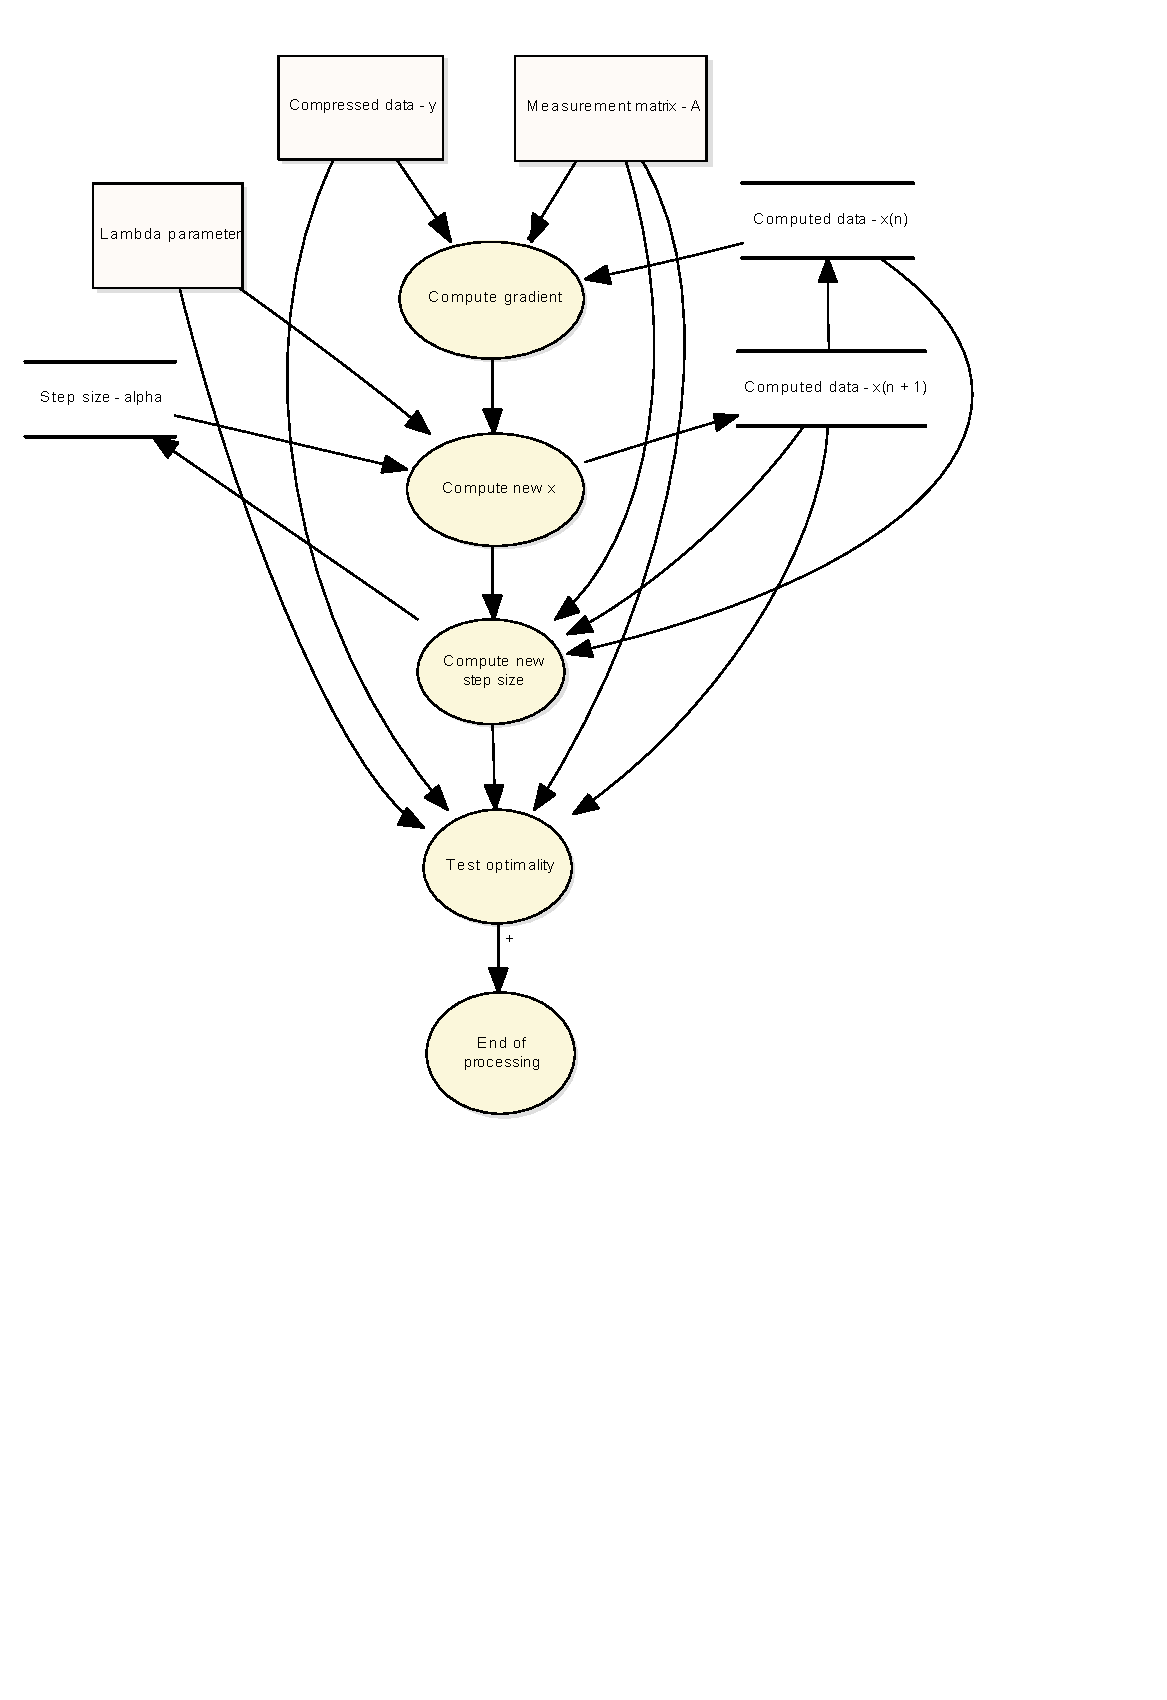
\includegraphics[scale=0.85]{obr/finalAlg.pdf}
		\end{center}
		\caption{Diagram finálního algoritmu}
		\label{fig:finalAlg}
	\end{figure}
\newpage
\addcontentsline{toc}{section}{Příloha C: Změna po jedné iteraci}
\section*{Příloha C: Změna po jedné iteraci}
\begin{figure}[!ht]
	\begin{center}
		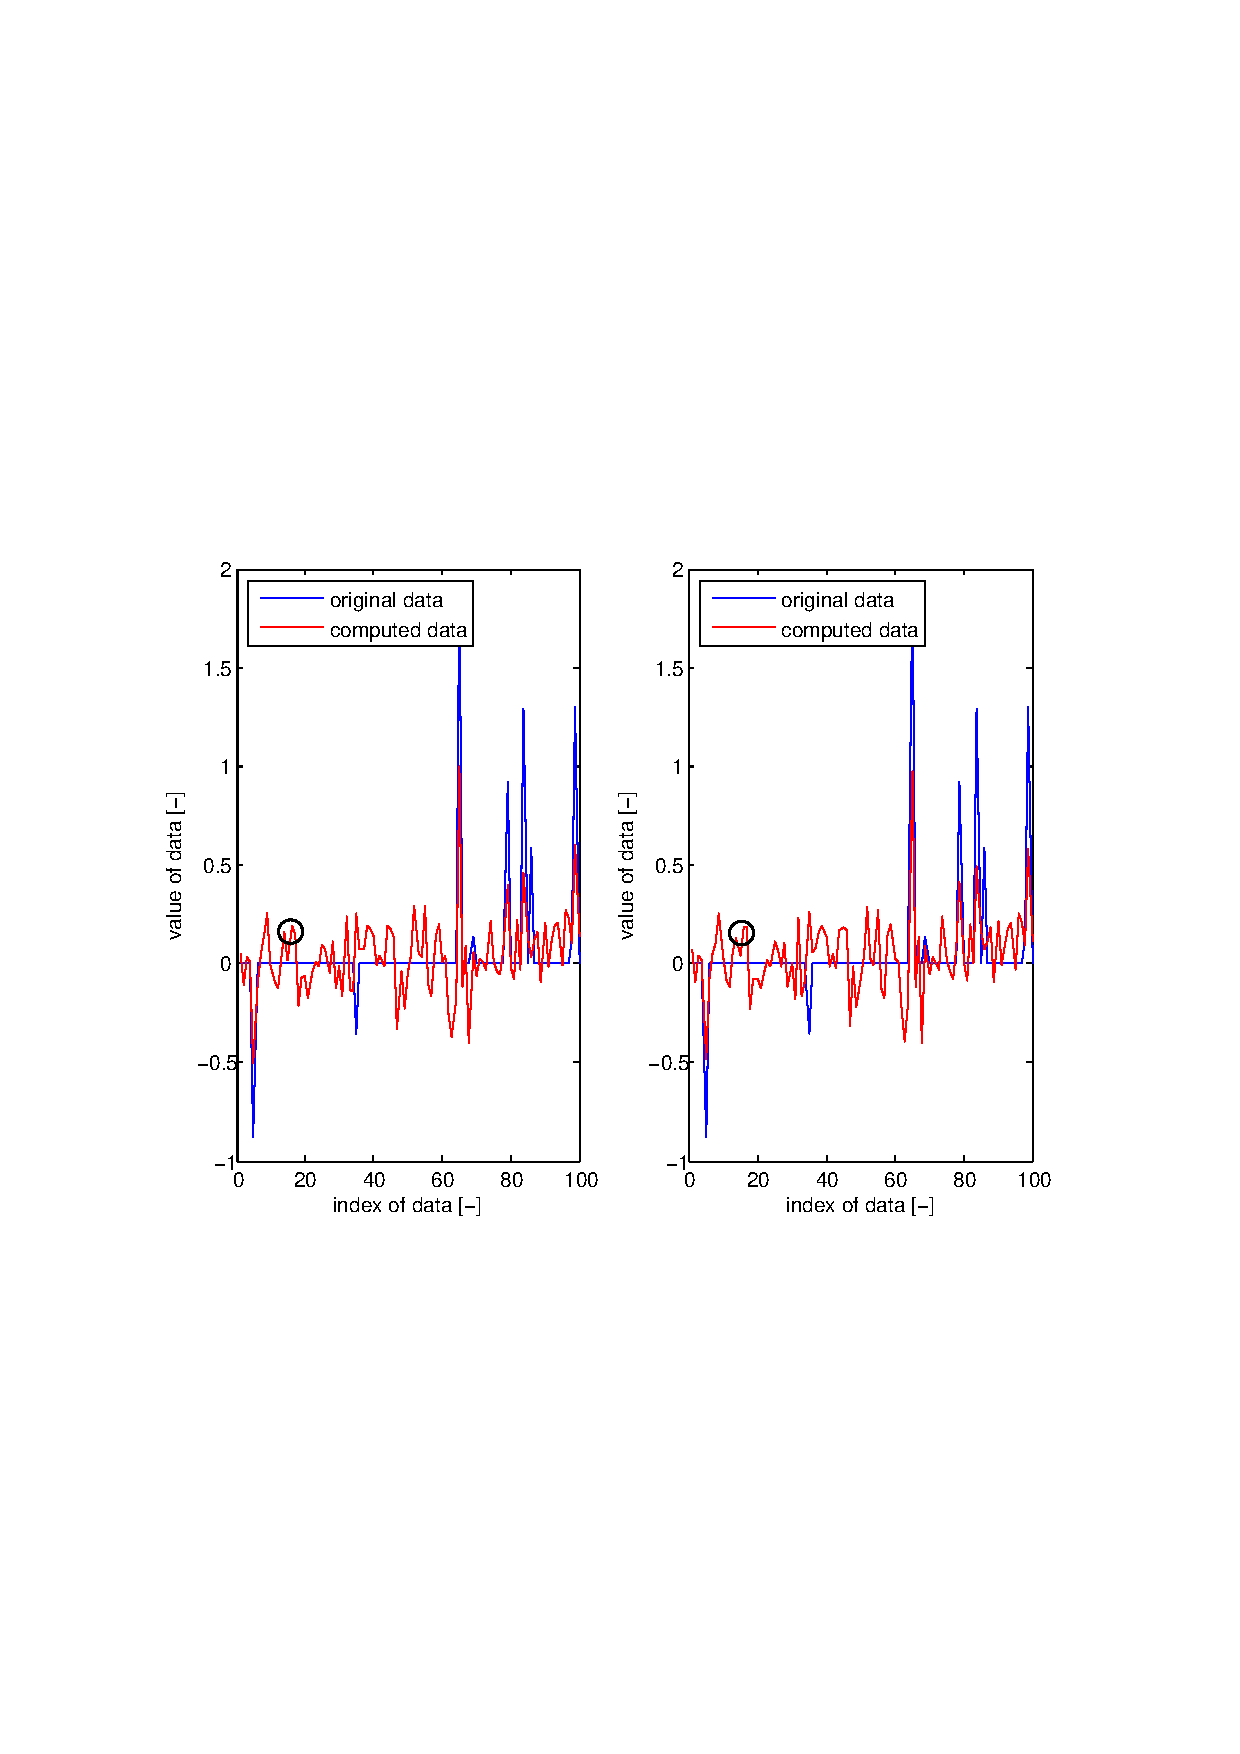
\includegraphics[scale=1]{obr/diff1.pdf}
		\end{center}
		\caption{Změna po jedné iteraci}
		\label{fig:diff1}
		\end{figure}
\newpage
\addcontentsline{toc}{section}{Příloha D: Změna po 300 iteracích}
\section*{Příloha D: Změna po 300 iteracích}
\begin{figure}[!ht]
	\begin{center}
		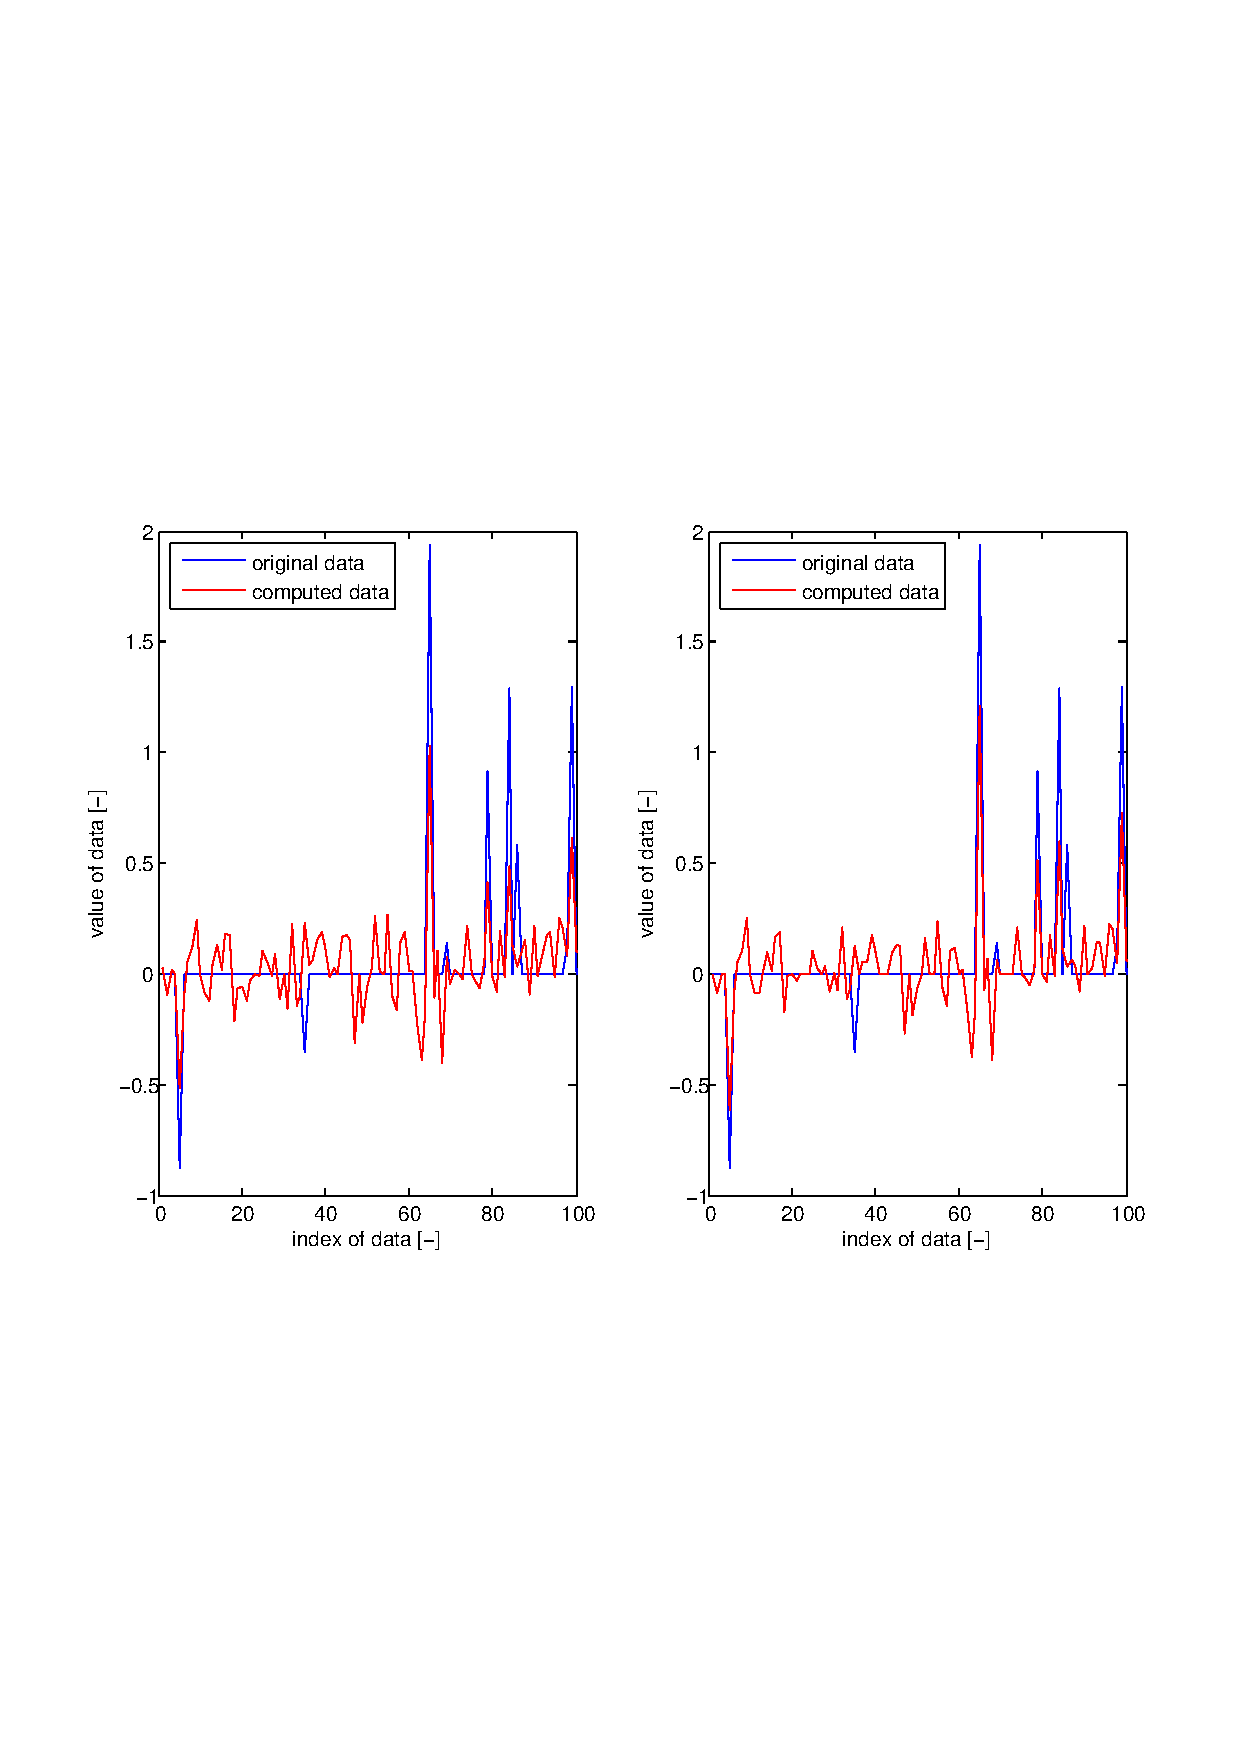
\includegraphics[scale=0.9]{obr/diff300.pdf}
	\end{center}
	\caption{Změna po 300 iteracích}
	\label{fig:diff300}
\end{figure}  
\end{document}
